\documentclass[a4paper, english, cleveref]{lipics-v2021}
\usepackage{booktabs}
\usepackage{KITcolors}
\usepackage[algo2e,vlined]{algorithm2e}
\usepackage{tikz}
\usetikzlibrary{calc,positioning,decorations,decorations.pathmorphing}

\usepackage{pifont}
\newcommand{\cmark}{\ding{51}}
\newcommand{\xmark}{\ding{55}}

\newcommand{\getAngle}[2]{%
    \pgfmathanglebetweenpoints{\pgfpointanchor{#1}{center}}
    {\pgfpointanchor{#2}{center}}
    \global\let\myangle\pgfmathresult % we need a global macro
}

\newcommand*{\elimtree}{\mathtt{ET}}
\newcommand*{\dist}{\mathcal{D}}
\newcommand*{\gchu}{G^{\uparrow}}
\newcommand*{\gchd}{G^{\downarrow}}
\newcommand*{\rgchd}{\overleftarrow{G^{\downarrow}}}
\newcommand*{\rgchu}{\overleftarrow{G^{\uparrow}}}
\newcommand*{\echu}{E^{\uparrow}}
\newcommand*{\echd}{E^{\downarrow}}
\newcommand*{\rechd}{\overleftarrow{E^{\downarrow}}}
\newcommand*{\rechu}{\overleftarrow{E^{\uparrow}}}
\newcommand*{\lchu}{\mathtt{l}^{\uparrow}}
\newcommand*{\lchd}{\mathtt{l}^{\downarrow}}
\newcommand*{\rlchd}{\overleftarrow{\mathtt{l}^{\downarrow}}}
\newcommand*{\rlchu}{\overleftarrow{\mathtt{l}^{\uparrow}}}

\bibliographystyle{plainurl}
\usetikzlibrary{backgrounds}

\title{Customizable Contraction Hierarchies with~Turn~Costs}

\author{Valentin Buchhold}{Karlsruhe Institute of Technology, Germany}{}{}{}
\author{Dorothea Wagner}{Karlsruhe Institute of Technology, Germany}{}{}{}
\author{Tim Zeitz}{Karlsruhe Institute of Technology, Germany}{}{}{}
\author{Michael Zündorf}{Karlsruhe Institute of Technology, Germany}{}{}{}

\authorrunning{V. Buchhold, D. Wagner, T. Zeitz, and M. Zündorf}
\Copyright{Valentin Buchhold, Dorothea Wagner, Tim Zeitz, and Michael Zündorf}

\ccsdesc[500]{Theory of computation~Shortest paths}
\ccsdesc[300]{Mathematics of computing~Graph algorithms}
\ccsdesc[500]{Applied computing~Transportation}

\keywords{Turn costs, realistic road networks, customizable contraction hierarchies, route planning, shortest paths}
\acknowledgements{We thank Peter Vortisch for providing the Stuttgart instance. We are also grateful to Transport for London (TfL) for permitting us to use their data, and to PTV AG for providing the London data. Further information about the London instance is provided by Tony Dichev (tonydichev@tfl.gov.uk).}
\nolinenumbers

%Editor-only macros:: begin (do not touch as author)%%%%%%%%%%%%%%%%%%%%%%%%%%%%%%%%%%
\EventEditors{Dennis Huisman and Christos D. Zaroliagis}
\EventNoEds{2}
\EventLongTitle{20th Symposium on Algorithmic Approaches for Transportation Modelling, Optimization, and Systems (ATMOS 2020)}
\EventShortTitle{ATMOS 2020}
\EventAcronym{ATMOS}
\EventYear{2020}
\EventDate{September 7--8, 2020}
\EventLocation{Pisa, Italy (Virtual Conference)}
\EventLogo{}
\SeriesVolume{85}
\ArticleNo{9}
%%%%%%%%%%%%%%%%%%%%%%%%%%%%%%%%%%%%%%%%%%%%%%%%%%%%%%

\begin{document}

\maketitle

\begin{abstract}
  We incorporate turn restrictions and turn costs into the route planning algorithm customizable contraction hierarchies (CCH). There are two common ways to represent turn costs and restrictions. The edge-based model expands the network so that road segments become vertices and allowed turns become edges. The compact model keeps intersections as vertices, but associates a turn table with each vertex. Although CCH can be used as is on the edge-based model, the performance of preprocessing and customization is severely affected. While the expanded network is only three times larger, both preprocessing and customization time increase by up to an order of magnitude. In this work, we carefully engineer CCH to exploit different properties of the expanded graph. We reduce the increase in customization time from up to an order of magnitude to a factor of about 3. The increase in preprocessing time is reduced even further. Moreover, we present a CCH variant that works on the compact model, and show that it performs worse than the variant on the edge-based model. Surprisingly, the variant on the edge-based model even uses less space than the one on the compact model, although the compact model was developed to keep the space requirement low.
\end{abstract}

\section{Introduction}

CCH faster but CRP more flexible/extensible than CCH
In this chapter, we review recent advances on CCH, propose additional improvements (refinements) and demonstrate practical feasibility.
In this chapter we do not propose a new technique for dynamic routing.
% CRP practical
% combine incremental contributions to build full routing framework
% (C)CH-Pot missing ingredient
Rather, we review and improve on recent advances for Customizable Contraction Hierarchies and show how to bring them all together to build a fully-fledged practical routing framework.

Motivated by computing driving directions, the last two decades have seen intense research on speedup techniques~\cite{BastDGMPSWW16} for Dijkstra's shortest-path algorithm~\cite{Dijkstra59}, which rely on a slow preprocessing phase to enable fast queries. Almost all previous experimental studies (e.g., \cite{GoldbergH05, HilgerKMS09, Lauther09, DibbeltSW16, Gutman04, AbrahamDGW11, ArzLS13, BastFSS07}) are restricted to the simplified model, where vertices represent intersections, edges represent road segments, and turn costs are ignored. While it has been widely believed that turn restrictions and turn costs are easy to incorporate, Delling et al.~\cite{DellingGPW17} show that most algorithms have a significant performance penalty. For long-range queries, one may argue that turn costs are negligible. When analyzing intracity traffic~\cite{BuchholdSW19, SchneckN20} or dispatching autonomous vehicles operating within a particular city~\cite{BischoffM16, BischoffMN17}, however, taking turn costs into account is of utmost importance.

A fairly recent development in the area of route planning are customizable speedup techniques, which split preprocessing into a slow metric-independent part, taking only the network structure into account, and a fast metric-dependent part (the \emph{customization}), incorporating edge costs (the \emph{metric}). Customizable route planning (CRP)~\cite{DellingGPW17} and customizable contraction hierarchies (CCH)~\cite{DibbeltSW16} are the most prominent among them, and are both used in commercial and research software. While CRP was developed with turn costs in mind, CCH was not. In this work, we incorporate turn restrictions and turn costs into CCH.

\subparagraph*{Related Work}

Turns can be encoded into the network structure by expanding the network so that road segments become vertices and allowed turns become edges~\cite{Caldwell61, Winter02}. This is known as the \emph{edge-based model}~\cite{BastDGMPSWW16}. While any speedup technique can work on an expanded network, some are more robust than others~\cite{DellingGPW17}. We are aware of two algorithms that have been tailored to handle turns. First, Geisberger and Vetter~\cite{GeisbergerV11} present a turn-aware version of (non-customizable) contraction hierarchies (CH)~\cite{GeisbergerSSV12}. Second, Delling et al.~\cite{DellingGPW11} develop CRP with turns in mind. Both independently proposed a different turn representation. The \emph{compact model} keeps intersection as vertices, but associates a \emph{turn table} with each vertex.

\subparagraph*{Our Contribution}

The contribution of this work is twofold. First, we propose several optimizations that accelerate CCH on the edge-based model by exploiting properties of the expanded network (\Cref{sec:cch-on-edge-based-model}). We reduce the increase in customization time from up to an order of magnitude to a factor of about three (which is reasonable since the expanded network is three times larger than the original network, which ignores turn costs). The increase in preprocessing time is reduced even further.

Second, we introduce a CCH variant that works on the compact model, and discuss various issues we found. An extensive experimental evaluation shows that the edge-based variant significantly outperforms the compact variant (\Cref{sec:experiments}). Surprisingly, the variant on the edge-based model even uses less space than the one on the compact model.

\subparagraph*{Outline}

\Cref{sec:preliminaries} formally defines the problem we solve and has background information. \Cref{sec:cch-on-edge-based-model} presents optimizations that accelerate CCH on the edge-based model.
Blub introduces a CCH variant that works on the compact model. \Cref{sec:experiments} presents an extensive experimental evaluation of both variants. \Cref{sec:conclusion} concludes with final remarks.

\section{Preliminaries}
\label{sec:preliminaries}

We are given a directed graph~$G = (V, E)$ where vertices represent intersections and edges represent roads. A cost function~$\ell: E \to \mathbb{R}_{\ge 0}$ assigns an arbitrary cost to each edge. We are also given two functions $r: E \times E \to \{0, 1\}$ and $c: E \times E \to \mathbb{R}_{\ge 0} \cup \{\infty\}$. If $r(e, f) = 0$, the head of $e$ is the tail of $f$ and the turn from $e$ to $f$ is allowed. The cost of the turn is given by $c(e, f)$. Note that $r$ and $c$ have to be \emph{consistent}, i.e., $r(e, f) = 1$ implies $c(e, f) = \infty$. Since $r$ depends on the network topology, it is part of the input to the preprocessing phase. The turn cost function~$c$ is part of the input to the customization phase since it depends on the current traffic situation and personal preferences.

A path $P$ from a point along an edge $e_0$ to a point along an edge $e_k$ is a triple that consists of a sequence of edges $\langle e_0, \dots, e_k \rangle$ with $r(e_i, e_{i + 1}) = 0$, a real-valued offset $o_0 \in [0, 1]$ on $e_0$, and a real-valued offset $o_k \in [0, 1]$ on $e_k$. The cost of a path is the sum of the costs of its constituent edges and turns, i.e., $\ell(P) = (1 - o_0) \cdot \ell(e_0) + \sum_{i = 1}^k (c(e_{i - 1}, e_i) + \ell(e_i)) - (1 - o_k) \cdot \ell(e_k)$. Given a source edge $e_s$ with offset $o_s$ and a target edge $e_t$ with offset $o_t$, the problem we consider is computing a shortest path from the start point along $e_s$ to the end point along $e_t$. For simplicity, we assume that $o_s = 1$ and $o_t = 1$ in the rest of this paper.

In the following, we discuss both common ways to represent turn costs and restrictions. After that, we describe Dijkstra's algorithm and CH, both on standard graphs (simplified or edge-based graphs) and on compact graphs. We also discuss CCH on the simplified model.

\subsection{Turn Representation}

The \emph{simplified model} ignores turn costs and restrictions; see \cref{fig:turn-representation} (left). To actually incorporate them, there are two common ways. We explain each in turn.

\begin{figure}[tb]
  \hfill
  \begin{tikzpicture}
  [junction/.style={fill=KITblack!5},
   edge/.style={>=stealth, ->, shorten >=1pt, shorten <=1pt},
   original edge/.style={edge, draw=black},
   baseline=(current bounding box.north)]

  \def\JunctionRadius{4ex}
  \pgfmathsetmacro{\Offset}{asin(1ex / \JunctionRadius)}

  \def\Name{J}
  \draw [junction] circle [radius=\JunctionRadius];
  \coordinate (\Name-E-en) at (  0 + \Offset:\JunctionRadius) {};
  \coordinate (\Name-W-en) at (180 + \Offset:\JunctionRadius) {};
  \coordinate (\Name-S-en) at (270          :\JunctionRadius) {};

  \coordinate (\Name-E-ex) at (  0 - \Offset:\JunctionRadius) {};
  \coordinate (\Name-N-ex) at ( 90          :\JunctionRadius) {};
  \coordinate (\Name-W-ex) at (180 - \Offset:\JunctionRadius) {};

  \path (J-E-ex) edge [original edge, ->] +( \JunctionRadius,0);
  \path (J-N-ex) edge [original edge, ->] +(0, \JunctionRadius);
  \path (J-W-ex) edge [original edge, ->] +(-\JunctionRadius,0);

  \path (J-E-en) edge [original edge, <-] +( \JunctionRadius,0);
  \path (J-W-en) edge [original edge, <-] +(-\JunctionRadius,0);
  \path (J-S-en) edge [original edge, <-] +(0,-\JunctionRadius);
\end{tikzpicture}
\hfill
  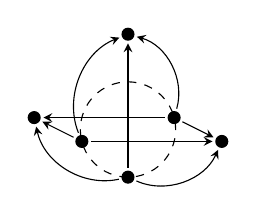
\begin{tikzpicture}
  [junction/.style={fill=KITblack!5},
   point/.style={draw, circle, inner sep=0pt, minimum size=1ex},
   entry/.style={point, fill=black},
   exit/.style={point, fill=white},
   edge/.style={>=stealth, ->, shorten >=1pt, shorten <=1pt},
   original edge/.style={edge, draw=black},
   baseline=(current bounding box.north)]

  \def\JunctionRadius{4ex}
  \pgfmathsetmacro{\Offset}{asin(1ex / \JunctionRadius)}

  \def\Name{J}
  \draw [dashed] circle [radius=\JunctionRadius];
  \node [entry] (\Name-E-en) at (  0 + \Offset:\JunctionRadius) {};
  \node [entry] (\Name-W-en) at (180 + \Offset:\JunctionRadius) {};
  \node [entry] (\Name-S-en) at (270          :\JunctionRadius) {};

  \node [entry, shift={( \JunctionRadius,0)}] (\Name-E-ex) at (  0 - \Offset:\JunctionRadius) {};
  \node [entry, shift={(0, \JunctionRadius)}] (\Name-N-ex) at ( 90          :\JunctionRadius) {};
  \node [entry, shift={(-\JunctionRadius,0)}] (\Name-W-ex) at (180 - \Offset:\JunctionRadius) {};

  \path (\Name-E-en) edge [original edge, ->] (\Name-E-ex);
  \path (\Name-E-en) edge [original edge, ->, bend right=45] (\Name-N-ex);
  \path (\Name-E-en) edge [original edge, ->] (\Name-W-ex);

  \path (\Name-W-en) edge [original edge, ->] (\Name-E-ex);
  \path (\Name-W-en) edge [original edge, ->, bend left=45] (\Name-N-ex);
  \path (\Name-W-en) edge [original edge, ->] (\Name-W-ex);

  \path (\Name-S-en) edge [original edge, ->, bend right=45] (\Name-E-ex);
  \path (\Name-S-en) edge [original edge, ->] (\Name-N-ex);
  \path (\Name-S-en) edge [original edge, ->, bend left=45] (\Name-W-ex);
\end{tikzpicture}
\hfill
  \begin{tikzpicture}
  [junction/.style={fill=KITblack!5},
   point/.style={draw, circle, inner sep=0pt, minimum size=1ex},
   entry/.style={point, fill=black},
   exit/.style={point, fill=white},
   edge/.style={>=stealth, ->, shorten >=1pt, shorten <=1pt},
   original edge/.style={edge, draw=black},
   turn edge/.style={edge, draw=KITgreen},
   baseline=(current bounding box.north)]

  \def\JunctionRadius{4ex}
  \pgfmathsetmacro{\Offset}{asin(1ex / \JunctionRadius)}

  % Looseness factors for the various turn types.
  \def\RightTurn  {1}
  \def\ThroughMove{1}
  \def\LeftTurn   {1}
  \def\UTurn      {2}

  \def\Name{J}
  \draw [junction] circle [radius=\JunctionRadius];
  \node [entry] (\Name-E-en) at (  0 + \Offset:\JunctionRadius) {};
  \node [entry] (\Name-W-en) at (180 + \Offset:\JunctionRadius) {};
  \node [entry] (\Name-S-en) at (270          :\JunctionRadius) {};

  \node [exit] (\Name-E-ex) at (  0 - \Offset:\JunctionRadius) {};
  \node [exit] (\Name-N-ex) at ( 90          :\JunctionRadius) {};
  \node [exit] (\Name-W-ex) at (180 - \Offset:\JunctionRadius) {};

  \path (\Name-E-en) edge [turn edge, out=180, in=180, looseness=\UTurn      ] (\Name-E-ex);
  \path (\Name-E-en) edge [turn edge, out=180, in=270, looseness=\RightTurn  ] (\Name-N-ex);
  \path (\Name-E-en) edge [turn edge, out=180, in=  0, looseness=\ThroughMove] (\Name-W-ex);

  \path (\Name-W-en) edge [turn edge, out=0, in=180, looseness=\ThroughMove] (\Name-E-ex);
  \path (\Name-W-en) edge [turn edge, out=0, in=270, looseness=\LeftTurn   ] (\Name-N-ex);
  \path (\Name-W-en) edge [turn edge, out=0, in=  0, looseness=\UTurn      ] (\Name-W-ex);

  \path (\Name-S-en) edge [turn edge, out=90, in=180, looseness=\RightTurn  ] (\Name-E-ex);
  \path (\Name-S-en) edge [turn edge, out=90, in=270, looseness=\ThroughMove] (\Name-N-ex);
  \path (\Name-S-en) edge [turn edge, out=90, in=  0, looseness=\LeftTurn   ] (\Name-W-ex);

  \path (J-E-ex) edge [original edge, ->] +( \JunctionRadius,0);
  \path (J-N-ex) edge [original edge, ->] +(0, \JunctionRadius);
  \path (J-W-ex) edge [original edge, ->] +(-\JunctionRadius,0);

  \path (J-E-en) edge [original edge, <-] +( \JunctionRadius,0);
  \path (J-W-en) edge [original edge, <-] +(-\JunctionRadius,0);
  \path (J-S-en) edge [original edge, <-] +(0,-\JunctionRadius);
\end{tikzpicture}
\hfill\hspace{0pt}
  \caption{Turn representations (from left): simplified model, edge-based model, compact model.}
  \label{fig:turn-representation}
\end{figure}

\subparagraph*{Edge-based Model}

The \emph{edge-based model}~\cite{Caldwell61, Winter02} expands the network so that road segments become vertices and allowed turns become edges; see \cref{fig:turn-representation} (middle) for an example. More precisely, the edge-based graph~$G_e = (V_e, E_e)$ is obtained from $G$ as follows. The vertices of $G_e$ are the edges of $G$, i.e, $V_e = E$. The edges of $G_e$ are the allowed turns of $G$, i.e., $E_e = \{(e, f): e, f \in E, r(e, f) = 0\}$. The cost of an edge~$(e, f) \in E_e$ is defined as $\ell_e(e, f) = c(e, f) + \ell(f)$. The main advantage of the edge-based model is that most route planning algorithms can be used as is on it, without further modifications.

\subparagraph*{Compact Model}

The \emph{compact model}~\cite{GeisbergerV11, DellingGPW17} keeps intersections as vertices, but associates a $p \times q$ \emph{turn table}~$T_v$ with each vertex~$v$, where $p$ and $q$ are the numbers of incoming and outgoing edges, respectively. The entry~$T_v(i, j)$ represents the cost of the turn from the $i$-th incoming edge~$e$ to the $j$-th outgoing edge~$f$, i.e., $T_v(i, j) = c(e, f)$. For each edge~$(v, w)$, its tail corresponds to an \emph{exit point} at $v$ and its head corresponds to an \emph{entry point} at $w$. Note that the entry points in the compact model translate directly to the vertices in the edge-based model; see \cref{fig:turn-representation} (right) for an example. We denote by $v|i$ the $i$-th exit (or entry) point at $v$ and by $(v|i, w|j)$ the edge whose tail corresponds to the $i$-th exit point at $v$ and whose head corresponds to the $j$-th entry point at $w$. The main advantage of the compact model is its low space overhead since turn tables can be shared among vertices (the number of distinct turn tables for continental instances such as the road network of Western Europe used in our experiments is in the thousands rather than millions~\cite{DellingGPW17}).

\subsection{Dijkstra's Algorithm}

\emph{Dijkstra's algorithm}~\cite{Dijkstra59} computes the shortest-path distances from a source vertex~$s$ to all other vertices. For each vertex~$v$, it maintains a \emph{distance label}~$d(v)$, which represents the cost of the shortest path from $s$ to $v$ seen so far. Moreover, it maintains an addressable priority queue~$Q$~\cite{SandersMDD19} of vertices, using their distance labels as keys. Initially, $d(s) = 0$ for the source~$s$, $d(v) = \infty$ for each vertex~$v \ne s$, and $Q = \{s\}$.

The algorithm repeatedly extracts a vertex~$v$ with minimum distance label from the queue and \emph{settles} it by \emph{relaxing} its outgoing edges~$(v, w)$. To relax an edge~$e = (v, w)$, the path from $s$ to $w$ via $v$ is compared with the shortest path from $s$ to $w$ found so far. More precisely, if $d(v) + \ell(e) < d(w)$, the algorithm sets $d(w) = d(v) + \ell(e)$ and inserts $w$ into the queue. It stops when the queue becomes empty. Note that Dijkstra's algorithm has the label-setting property, i.e., each vertex is settled at most once. Therefore, when computing a point-to-point shortest path from a source~$s$ to a target~$t$, we can stop when $t$ is settled.

\subparagraph*{On the Compact Model}

For correctness, we must work on entry points instead of vertices. That is, we maintain a distance label~$d(v|i)$ for each entry point~$v|i$ and a queue~$Q$ of unsettled entry points. Initially, $d(s|i) = 0$ for the entry point~$s|i$ corresponding to the head of the source edge, $d(v|j) = \infty$ for all other entry points~$v|j$, and $Q = \{s|i\}$. To settle an entry point~$v|i$, we set $d(w|k) = \min\{d(w|k), d(v|i) + T_v(i, j) + \ell(e)\}$ for each outgoing edge~$e = (v|j, w|k)$. Each entry point is settled at most once, however, each vertex can be visited multiple times. Note that Dijkstra's algorithm on the compact model essentially simulates the execution on the edge-based model.

\subsection{Contraction Hierarchies}

\emph{Contraction hierarchies} (CH)~\cite{GeisbergerSSV12} is a two-phase speedup technique to accelerate point-to-point shortest-path computations, which exploits the inherent hierarchy of road networks. To differentiate it from customizable CH, we sometimes call it \emph{weighted} or \emph{standard} CH. The preprocessing phase heuristically orders the vertices by importance, and \emph{contracts} them from least to most important. Intuitively, vertices that hit many shortest paths are considered more important, such as vertices on highways. To contract a vertex~$v$, it is temporarily removed from the graph, and \emph{shortcut} edges are added between its neighbors to preserve distances in the remaining graph (without $v$). Note that a shortcut is only needed if it represents the only shortest path between its endpoints, which can be checked by running a \emph{witness search} (local Dijkstra) between its endpoints.

The query phase performs a bidirectional Dijkstra on the augmented graph that only relaxes edges leading to vertices of higher \emph{ranks} (importance). The stall-on-demand~\cite{GeisbergerSSV12} optimization prunes the search at any vertex~$v$ with a suboptimal distance label, which can be checked by looking at upward edges coming into $v$.

\subparagraph*{On the Compact Model}

Recall that we must maintain and compute distance labels for entry points (rather than vertices) in the compact model. Therefore, when contracting a vertex~$v$, we need to preserve the distances between all entry points in the remaining graph (without~$v$). In general, we cannot avoid self-loops and parallel edges. See \cref{fig:contract-on-compact-model} for an example. Contracting vertex~$v'$ creates a self-loop at vertex~$v$, because the through movement from $v$'s left entry point to its right exit point is costlier than the path via $v'$. Analogously, contracting $v$ results in two parallel edges between vertices $u$ and $w$. When entering $u$ from the west and leaving $w$ to the east, the shortest path is via $v$. In contrast, when entering $u$ from the north and leaving $w$ to the north, it is better to traverse the edge between $u$ and $w$.

Self-loops make the computation of shortcuts more complicated. Each shortcut is no longer a concatenation of exactly two edges, but can also include one or more self-loops at the middle vertex. For example, in \cref{fig:contract-on-compact-model}, the shortcut between $u$ and $w$ includes the self-loop at $v$. Therefore, Geisberger and Vetter~\cite{GeisbergerV11} use the witness search not only to decide whether a shortcut is necessary but also to compute the cost of the shortcut.

More precisely, to contract a vertex~$v$, they run a witness search for each exit point~$u|i$ such that there is at least one incoming edge~$(u|i, v)$. Initially, they set $d(v'|j) = \ell(e)$ for each edge~$e = (u|i, v'|j)$. Moreover, each entry point~$v'|j$ is inserted into the queue. The witness search stops when each entry point~$w|l$ such that there is at least one edge~$(v, w|l)$ has been settled. A shortcut~$s = (u|i, w|l)$ is only added if it is built from an edge~$(u|i, v)$, zero or more self-loops at $v$, and an edge~$(v, w|l)$. The shortcut has cost~$\ell(s) = d(w|l)$.

The query phase runs a bidirectional version of the turn-aware Dijkstra described above, but does not relax edges leading to lower-ranked vertices. Note that the stall-on-demand optimization can also be applied in the compact model~\cite{GeisbergerV11}.

\begin{figure}[tb]
  \begin{tikzpicture}
  [make transparent/.style={nearly transparent, transparency group},
   junction/.style={fill=KITblack!5},
   point/.style={draw, circle, inner sep=0pt, minimum size=1ex},
   entry/.style={point, fill=black},
   exit/.style={point, fill=white},
   edge/.style={>=stealth, ->, shorten >=1pt, shorten <=1pt},
   original edge/.style={edge, draw=black},
   turn edge/.style={edge, draw=KITgreen},
   shortcut edge/.style={edge, draw=KITblue}]

  \def\JunctionRadius{4ex}
  \def\JunctionMargin{1.5 * \JunctionRadius}
  \pgfmathsetmacro{\Offset}{asin(1ex / \JunctionRadius)}

  % Looseness factors for the various turn types.
  \def\RightTurn  {1}
  \def\ThroughMove{1}
  \def\LeftTurn   {1}
  \def\UTurn      {2}

  % North-eastern junction.
  \begin{scope}[shift={(60:2 * \JunctionRadius + \JunctionMargin)}]
    \def\Name{NE}
    \draw [junction] circle [radius=\JunctionRadius];
    \node at (-135:\JunctionRadius / 2) {$w$};

    \node [entry] (\Name-W-en) at (180:\JunctionRadius) {};
    \node [entry] (\Name-S-en) at (270:\JunctionRadius) {};

    \node [exit] (\Name-E-ex) at ( 0:\JunctionRadius) {};
    \node [exit] (\Name-N-ex) at (90:\JunctionRadius) {};

    \path (\Name-W-en) edge [turn edge, out=0, in=180, looseness=\ThroughMove] (\Name-E-ex);
    \path (\Name-W-en) edge [turn edge, out=0, in=270, looseness=\LeftTurn   ] (\Name-N-ex);

    \path (\Name-S-en) edge [turn edge, out=90, in=180, looseness=\RightTurn  ] (\Name-E-ex);
    \path (\Name-S-en) edge [turn edge, out=90, in=270, looseness=\ThroughMove] (\Name-N-ex);

    \path (NE-E-ex) edge [original edge, ->] +(\JunctionMargin / 2,0);
    \path (NE-N-ex) edge [original edge, ->] +(0,\JunctionMargin / 2);
  \end{scope}

  % North-western junction.
  \begin{scope}[shift={(120:2 * \JunctionRadius + \JunctionMargin)}]
    \def\Name{NW}
    \draw [junction] circle [radius=\JunctionRadius];
    \node at (-45:\JunctionRadius / 2) {$u$};

    \node [entry] (\Name-N-en) at ( 90:\JunctionRadius) {};
    \node [entry] (\Name-W-en) at (180:\JunctionRadius) {};

    \node [exit] (\Name-E-ex) at (  0:\JunctionRadius) {};
    \node [exit] (\Name-S-ex) at (270:\JunctionRadius) {};

    \path (\Name-N-en) edge [turn edge, out=270, in=180, looseness=\LeftTurn   ] (\Name-E-ex);
    \path (\Name-N-en) edge [turn edge, out=270, in= 90, looseness=\ThroughMove] (\Name-S-ex);

    \path (\Name-W-en) edge [turn edge, out=0, in=180, looseness=\ThroughMove] (\Name-E-ex);
    \path (\Name-W-en) edge [turn edge, out=0, in= 90, looseness=\RightTurn  ] (\Name-S-ex);

    \path (NW-E-ex) edge [original edge, ->] (NE-W-en);

    \path (NW-N-en) edge [original edge, <-] +(0, \JunctionMargin / 2);
    \path (NW-W-en) edge [original edge, <-] +(-\JunctionMargin / 2,0);
  \end{scope}

  % Centered junction.
  \begin{scope}
    \def\Name{CC}
    \draw [junction] circle [radius=\JunctionRadius];
    \node at (90:\JunctionRadius / 2) {$v$};

    \node [entry] (\Name-W-en) at (180          :\JunctionRadius) {};
    \node [entry] (\Name-S-en) at (270 + \Offset:\JunctionRadius) {};

    \node [exit] (\Name-E-ex) at (  0          :\JunctionRadius) {};
    \node [exit] (\Name-S-ex) at (270 - \Offset:\JunctionRadius) {};

    \path (\Name-W-en) edge [turn edge, out=0, in=180, looseness=\ThroughMove] (\Name-E-ex);
    \path (\Name-W-en) edge [turn edge, out=0, in= 90, looseness=\RightTurn  ] (\Name-S-ex);

    \path (\Name-S-en) edge [turn edge, out=90, in=180, looseness=\RightTurn] (\Name-E-ex);
    \path (\Name-S-en) edge [turn edge, out=90, in= 90, looseness=\UTurn    ] (\Name-S-ex);

    \path (CC-E-ex) edge [original edge, ->, out=  0, in=270, looseness=0.75] (NE-S-en);
    \path (CC-W-en) edge [original edge, <-, out=180, in=270, looseness=0.75] (NW-S-ex);
  \end{scope}

  % Southern junction.
  \begin{scope}[shift={(270:2 * \JunctionRadius + \JunctionMargin)}]
    \def\Name{SS}
    \draw [junction] circle [radius=\JunctionRadius];
    \node {$v'$};
    \node [entry] (\Name-N-en) at (90 + \Offset:\JunctionRadius) {};
    \node [exit] (\Name-N-ex) at (90 - \Offset:\JunctionRadius) {};
    \path (\Name-N-en) edge [turn edge, out=270, in=270, looseness=\UTurn] (\Name-N-ex);
    \path (SS-N-ex) edge [original edge, ->] (CC-S-en);
    \path (SS-N-en) edge [original edge, <-] (CC-S-ex);
  \end{scope}
\end{tikzpicture}
\hfill
  \begin{tikzpicture}
  [make transparent/.style={nearly transparent, transparency group},
   junction/.style={fill=KITblack!5},
   point/.style={draw, circle, inner sep=0pt, minimum size=1ex},
   entry/.style={point, fill=black},
   exit/.style={point, fill=white},
   edge/.style={>=stealth, ->, shorten >=1pt, shorten <=1pt},
   original edge/.style={edge, draw=black},
   turn edge/.style={edge, draw=KITgreen},
   shortcut edge/.style={edge, draw=KITblue}]

  \def\JunctionRadius{4ex}
  \def\JunctionMargin{1.5 * \JunctionRadius}
  \pgfmathsetmacro{\Offset}{asin(1ex / \JunctionRadius)}

  % Looseness factors for the various turn types.
  \def\RightTurn  {1}
  \def\ThroughMove{1}
  \def\LeftTurn   {1}
  \def\UTurn      {2}

  % North-eastern junction.
  \begin{scope}[shift={(60:2 * \JunctionRadius + \JunctionMargin)}]
    \def\Name{NE}
    \draw [junction] circle [radius=\JunctionRadius];
    \node at (-135:\JunctionRadius / 2) {$w$};

    \node [entry] (\Name-W-en) at (180:\JunctionRadius) {};
    \node [entry] (\Name-S-en) at (270:\JunctionRadius) {};

    \node [exit] (\Name-E-ex) at ( 0:\JunctionRadius) {};
    \node [exit] (\Name-N-ex) at (90:\JunctionRadius) {};

    \path (\Name-W-en) edge [turn edge, out=0, in=180, looseness=\ThroughMove] (\Name-E-ex);
    \path (\Name-W-en) edge [turn edge, out=0, in=270, looseness=\LeftTurn   ] (\Name-N-ex);

    \path (\Name-S-en) edge [turn edge, out=90, in=180, looseness=\RightTurn  ] (\Name-E-ex);
    \path (\Name-S-en) edge [turn edge, out=90, in=270, looseness=\ThroughMove] (\Name-N-ex);

    \path (NE-E-ex) edge [original edge, ->] +(\JunctionMargin / 2,0);
    \path (NE-N-ex) edge [original edge, ->] +(0,\JunctionMargin / 2);
  \end{scope}

  % North-western junction.
  \begin{scope}[shift={(120:2 * \JunctionRadius + \JunctionMargin)}]
    \def\Name{NW}
    \draw [junction] circle [radius=\JunctionRadius];
    \node at (-45:\JunctionRadius / 2) {$u$};

    \node [entry] (\Name-N-en) at ( 90:\JunctionRadius) {};
    \node [entry] (\Name-W-en) at (180:\JunctionRadius) {};

    \node [exit] (\Name-E-ex) at (  0:\JunctionRadius) {};
    \node [exit] (\Name-S-ex) at (270:\JunctionRadius) {};

    \path (\Name-N-en) edge [turn edge, out=270, in=180, looseness=\LeftTurn   ] (\Name-E-ex);
    \path (\Name-N-en) edge [turn edge, out=270, in= 90, looseness=\ThroughMove] (\Name-S-ex);

    \path (\Name-W-en) edge [turn edge, out=0, in=180, looseness=\ThroughMove] (\Name-E-ex);
    \path (\Name-W-en) edge [turn edge, out=0, in= 90, looseness=\RightTurn  ] (\Name-S-ex);

    \path (NW-E-ex) edge [original edge, ->] (NE-W-en);

    \path (NW-N-en) edge [original edge, <-] +(0, \JunctionMargin / 2);
    \path (NW-W-en) edge [original edge, <-] +(-\JunctionMargin / 2,0);
  \end{scope}

  % Centered junction.
  \begin{scope}
    \def\Name{CC}
    \draw [junction] circle [radius=\JunctionRadius];
    \node at (90:\JunctionRadius / 2) {$v$};

    \node [entry] (\Name-W-en) at (180          :\JunctionRadius) {};
    \node [entry] (\Name-S-en) at (270 + \Offset:\JunctionRadius) {};

    \node [exit] (\Name-E-ex) at (  0          :\JunctionRadius) {};
    \node [exit] (\Name-S-ex) at (270 - \Offset:\JunctionRadius) {};

    \path (\Name-W-en) edge [turn edge, out=0, in=180, looseness=\ThroughMove] (\Name-E-ex);
    \path (\Name-W-en) edge [turn edge, out=0, in= 90, looseness=\RightTurn  ] (\Name-S-ex);

    \path (\Name-S-en) edge [turn edge, out=90, in=180, looseness=\RightTurn] (\Name-E-ex);
    \path (\Name-S-en) edge [turn edge, out=90, in= 90, looseness=\UTurn    ] (\Name-S-ex);

    \path (CC-E-ex) edge [original edge, ->, out=  0, in=270, looseness=0.75] (NE-S-en);
    \path (CC-W-en) edge [original edge, <-, out=180, in=270, looseness=0.75] (NW-S-ex);

    \path (CC-S-ex) edge [shortcut edge, ->, out=-75, in=180 + 60, relative, looseness=2] (CC-S-en);
  \end{scope}

  % Southern junction.
  \begin{scope}[shift={(270:2 * \JunctionRadius + \JunctionMargin)}, make transparent]
    \def\Name{SS}
    \draw [junction] circle [radius=\JunctionRadius];
    \node {$v'$};
    \node [entry] (\Name-N-en) at (90 + \Offset:\JunctionRadius) {};
    \node [exit] (\Name-N-ex) at (90 - \Offset:\JunctionRadius) {};
    \path (\Name-N-en) edge [turn edge, out=270, in=270, looseness=\UTurn] (\Name-N-ex);
    \path (SS-N-ex) edge [original edge, ->] (CC-S-en);
    \path (SS-N-en) edge [original edge, <-] (CC-S-ex);
  \end{scope}
\end{tikzpicture}
\hfill
  \begin{tikzpicture}
  [make transparent/.style={nearly transparent, transparency group},
   junction/.style={fill=KITblack!5},
   point/.style={draw, circle, inner sep=0pt, minimum size=1ex},
   entry/.style={point, fill=black},
   exit/.style={point, fill=white},
   edge/.style={>=stealth, ->, shorten >=1pt, shorten <=1pt},
   original edge/.style={edge, draw=black},
   turn edge/.style={edge, draw=KITgreen},
   shortcut edge/.style={edge, draw=KITblue}]

  \def\JunctionRadius{4ex}
  \def\JunctionMargin{1.5 * \JunctionRadius}
  \pgfmathsetmacro{\Offset}{asin(1ex / \JunctionRadius)}

  % Looseness factors for the various turn types.
  \def\RightTurn  {1}
  \def\ThroughMove{1}
  \def\LeftTurn   {1}
  \def\UTurn      {2}

  % North-eastern junction.
  \begin{scope}[shift={(60:2 * \JunctionRadius + \JunctionMargin)}]
    \def\Name{NE}
    \draw [junction] circle [radius=\JunctionRadius];
    \node at (-135:\JunctionRadius / 2) {$w$};

    \node [entry] (\Name-W-en) at (180:\JunctionRadius) {};
    \node [entry] (\Name-S-en) at (270:\JunctionRadius) {};

    \node [exit] (\Name-E-ex) at ( 0:\JunctionRadius) {};
    \node [exit] (\Name-N-ex) at (90:\JunctionRadius) {};

    \path (\Name-W-en) edge [turn edge, out=0, in=180, looseness=\ThroughMove] (\Name-E-ex);
    \path (\Name-W-en) edge [turn edge, out=0, in=270, looseness=\LeftTurn   ] (\Name-N-ex);

    \path (\Name-S-en) edge [turn edge, out=90, in=180, looseness=\RightTurn  ] (\Name-E-ex);
    \path (\Name-S-en) edge [turn edge, out=90, in=270, looseness=\ThroughMove] (\Name-N-ex);

    \path (NE-E-ex) edge [original edge, ->] +(\JunctionMargin / 2,0);
    \path (NE-N-ex) edge [original edge, ->] +(0,\JunctionMargin / 2);
  \end{scope}

  % North-western junction.
  \begin{scope}[shift={(120:2 * \JunctionRadius + \JunctionMargin)}]
    \def\Name{NW}
    \draw [junction] circle [radius=\JunctionRadius];
    \node at (-45:\JunctionRadius / 2) {$u$};

    \node [entry] (\Name-N-en) at ( 90:\JunctionRadius) {};
    \node [entry] (\Name-W-en) at (180:\JunctionRadius) {};

    \node [exit] (\Name-E-ex) at (  0:\JunctionRadius) {};
    \node [exit] (\Name-S-ex) at (270:\JunctionRadius) {};

    \path (\Name-N-en) edge [turn edge, out=270, in=180, looseness=\LeftTurn   ] (\Name-E-ex);
    \path (\Name-N-en) edge [turn edge, out=270, in= 90, looseness=\ThroughMove] (\Name-S-ex);

    \path (\Name-W-en) edge [turn edge, out=0, in=180, looseness=\ThroughMove] (\Name-E-ex);
    \path (\Name-W-en) edge [turn edge, out=0, in= 90, looseness=\RightTurn  ] (\Name-S-ex);

    \path (NW-E-ex) edge [original edge, ->] (NE-W-en);

    \path (NW-N-en) edge [original edge, <-] +(0, \JunctionMargin / 2);
    \path (NW-W-en) edge [original edge, <-] +(-\JunctionMargin / 2,0);

    \path (NW-S-ex) edge [shortcut edge, ->, out=-30, in=180 + 30, relative] (NE-S-en);
  \end{scope}

  % Centered junction.
  \begin{scope}[make transparent]
    \def\Name{CC}
    \draw [junction] circle [radius=\JunctionRadius];
    \node at (90:\JunctionRadius / 2) {$v$};

    \node [entry] (\Name-W-en) at (180          :\JunctionRadius) {};
    \node [entry] (\Name-S-en) at (270 + \Offset:\JunctionRadius) {};

    \node [exit] (\Name-E-ex) at (  0          :\JunctionRadius) {};
    \node [exit] (\Name-S-ex) at (270 - \Offset:\JunctionRadius) {};

    \path (\Name-W-en) edge [turn edge, out=0, in=180, looseness=\ThroughMove] (\Name-E-ex);
    \path (\Name-W-en) edge [turn edge, out=0, in= 90, looseness=\RightTurn  ] (\Name-S-ex);

    \path (\Name-S-en) edge [turn edge, out=90, in=180, looseness=\RightTurn] (\Name-E-ex);
    \path (\Name-S-en) edge [turn edge, out=90, in= 90, looseness=\UTurn    ] (\Name-S-ex);

    \path (CC-E-ex) edge [original edge, ->, out=  0, in=270, looseness=0.75] (NE-S-en);
    \path (CC-W-en) edge [original edge, <-, out=180, in=270, looseness=0.75] (NW-S-ex);

    \path (CC-S-ex) edge [shortcut edge, ->, out=-75, in=180 + 60, relative, looseness=2] (CC-S-en);
  \end{scope}

  % Southern junction.
  \begin{scope}[shift={(270:2 * \JunctionRadius + \JunctionMargin)}, make transparent]
    \def\Name{SS}
    \draw [junction] circle [radius=\JunctionRadius];
    \node {$v'$};
    \node [entry] (\Name-N-en) at (90 + \Offset:\JunctionRadius) {};
    \node [exit] (\Name-N-ex) at (90 - \Offset:\JunctionRadius) {};
    \path (\Name-N-en) edge [turn edge, out=270, in=270, looseness=\UTurn] (\Name-N-ex);
    \path (SS-N-ex) edge [original edge, ->] (CC-S-en);
    \path (SS-N-en) edge [original edge, <-] (CC-S-ex);
  \end{scope}
\end{tikzpicture}

  \caption{Vertex contraction on the compact model. Original edges are shown in black, turn edges are shown in green, and shortcut edges are shown in blue. Each original edge and each right-, left- and U-turn movement has cost~1. Each through movement has cost 10. Left: A subgraph before contraction. Middle: Contracting vertex~$v'$ creates a self-loop at $v$ (cost~3). Right: Contracting $v$ creates a shortcut edge between $u$ and $w$ (cost~7), resulting in two parallel edges between them.}
  \label{fig:contract-on-compact-model}
\end{figure}

\subsection{Customizable Contraction Hierarchies}

\emph{Customizable contraction hierarchies} (CCH)~\cite{DibbeltSW16} are a three-phase technique, splitting CH preprocessing into a relatively slow metric-independent phase and a much faster customization phase.
The metric-independent phase computes a \emph{separator decomposition}~\cite{BauerCRW16} of the unweighted graph, determines an associated \emph{nested dissection order}~\cite{George73} on the vertices, and contracts them in this order without running witness searches (which depend on the metric).
Therefore, it adds every potential shortcut.
The customization phase computes the costs of the edges in the hierarchy by processing them in bottom-up fashion.
To process an edge~$(u, w)$, it enumerates all triangles~$\{v, u, w\}$ where $v$ has lower rank than $u$ and $w$, and checks if the path $\langle u, v, w \rangle$ improves the cost of $(u, w)$. Alternatively, Buchhold et al.~\cite{BuchholdSW19} enumerate all triangles~$\{u, w, v'\}$ where $v'$ has higher rank than $u$ and $w$, and check if the path $\langle v', u, w \rangle$ improves the cost of $(v', w)$, accelerating customization by a factor of 2.

There are two known query algorithms.
First, one can run a standard CH search without modification.
In addition, Dibbelt et al.~\cite{DibbeltSW16} describe a query algorithm based on the \emph{elimination tree} of the augmented graph.
The parent of a vertex in the elimination tree is its lowest-ranked higher neighbor in the augmented graph.
Bauer et al.~\cite{BauerCRW16} prove that the ancestors of a vertex~$v$ in the elimination tree are exactly the set of vertices in the CH search space of $v$.
Hence, the elimination tree query algorithm explores the search space by traversing a path in the elimination tree, thereby avoiding a priority queue completely.
Buchhold et al.~\cite{BuchholdSW19} propose further optimizations for the elimination tree search, which achieve significant speedups for short- and mid-range queries.

\section{Algorithms}
% TODO metric
\subsection{Metric-Independent Preprocessing}

The metric-independent preprocessing phase works purely on the topology of the input network.
Since changes to this topology should be fairly rare, it is OK for this phase to take hours.
The algorithms used in this phase work with undirected graphs.
Therefore, initially, for any edge $uv \in E$ where $vu \notin E$, $vu$ is added to $E$ so the graph becomes bidirected.

\subsubsection{Ordering}

The most crucial step of the metric-independent preprocessing is to obtain a importance ordering.
In theory, any ordering suffices.
However, a good ordering is critical for the performance.
With bad orders it may even be impossible to compute the augmented graph.
As no witness search is possible without a weight function, all possible shortcuts will be inserted in the contraction step.
This corresponds to the minimal chordally completed supergraph.
With a bad ordering the number of additional edges in this supergraph can quickly become too much even for the main memory of high-end server machines.
This even happens with ``good'' CH orders.

Therefore, CCH are build on \emph{nested dissection orders} which are a very effective heuristic for elimination orders for small chordal supergraphs.
A nested dissection order is obtained by recursively computing small vertex separators which split the graph in two (or more) roughly balanced \emph{cells}.
The vertices in the separator get the highest ranks, i.e.\ appear last in the contraction order.
Removing these separator vertices leaves two (or more) disconnected cells.
To order the vertices in these cells, the algorithm is applied recursively.
The order within the separator vertices is arbitrary.
Luckily, vertices with high rank in this order also lie on many shortest paths.
All shortest paths from one cell to the other must use a vertex of the separator.
Thus, a nested dissection order is also a good CH order.
% sep decomp to order

% separators on road networks
Computing small balanced separators is an \textsf{NP}-hard problem.
Therefore, in general, one cannot expect to obtain small balanced separators efficiently.
% lot of research
Luckily, road networks have turned out to be relatively easily separable due to natural features such as rivers or mountain ranges.
InertialFlow~\cite{TODO} is an example of an extremely simple yet surprisingly effective partitioning algorithm for road networks.
For this algorithm, vertices are projected on geographic axis (the north-south axis for example), then the first and last quarter of vertices are contracted and then a minimum cut between these contracted vertices is computed.
Taking the vertices on one side of these cut edges yields a separator candidate.
Repeating this process for different axis and taking the smallest separator yields surprisingly good results.
More sophisticated algorithms for partitioning road networks have been developed, are available as open source and can be deployed as black box ordering algorithms.
A comprehensive review is beyond the scope of this work.
To the best of our knowledge, InertialFlowCutter, a combination of InertialFlow and FlowCutter, currently yields the best results.
See for a comprehensive experimental comparison.
We therefore use InertialFlowCutter orders for all experiments in this work.

To maximize cache efficiency, the contraction order should be derived as a DFS-post order on the tree of the separator decomposition.
This also ensures that the vertices of each cell form a consecutive range in the order.
InertialFlowCutter computes a BFS-post ordering.
We therefore reconstruct the separator decomposition and obtain a corresponding DFS-post order as described in Section~\ref{sec:reconstruct_sep_tree}

\subsubsection{Contraction}

% undirected/bidirected represented by only up
Once an importance ordering was obtained, the remaining part of the metric-independent preprocessing is to compute the topology of the augmented graph $G^+=(V, E^+)$.
Since the graph is fully bidirected ($\gchu = \rgchd$) it is sufficient to store every edge only at its lower ranked endpoint, i.e.\ maintain $\gchu$.
For cache efficiency in this and all following phases it is also crucial to permute the vertex IDs such that IDs equal the ranks.
This graph must contain \emph{every} shortcut edge which might be relevant for \emph{any} weight function.
Thus, the simplest way to construct this graph is to perform the classical CH preprocessing for the given order without any witness search, i.e.\ iterate over all vertices by ascending rank and ensure that a shortcut edge exists between any pair of upward neighbors of each vertex.
The result of this process is the minimal chordal supergraph of $G$ for which the importance ordering is a perfect elimination scheme.
Because the naive approach is rather expensive in terms of running time, the authors of~\cite{DibbeltSW16} propose a faster algorithm based on a quotient graph~\cite{TODO}.
However, this algorithm is rather complex.
Here, we describe a simpler and even faster algorithm, which so far has only been described in a Bachelor's thesis~\cite{TODO}.
It is heavily based on the linear time chordal graph recognition algorithm of~\cite{TODO}.

The algorithm iterates over all vertices in order of ascending rank.
Let $v$ be the current vertex and $N_{\gchu}(v)$ its upward neighborhood.
If this neighborhood is non-empty, the algorithm obtains the upward neighbor $u$ with minimal rank.
The remaining neighborhood $N_{\gchu}(v) \setminus u$ of $v$ is merged into the neighborhood of $u$, i.e.\ $N_{\gchu}(u) \gets N_{\gchu}(u) \cup N_{\gchu}(v) \setminus u$.
The result is the minimal chordal supergraph of $G$ induced by the nested dissection order.

This algorithm can be implemented by maintaining the neighborhood of each vertex in a dynamic array.
A theoretical worst-case running time of $\mathcal{O}(|V| + |\echu|)$ can be achieved by appending the neighborhoods without checking for duplicates and only performing the deduplication when extracting the minimally ranked upward neighbor.
See~\cite{TODO} for a proof of the running time and the correctness.
However, for a practical implementation, it is even more efficient to ensure that the neighborhoods never contain any duplicates and are always sorted by rank.
Merging neighborhoods can then be realized with a coordinated linear sweep.
The worst-case running time of this variant is slightly worse, but in practice, running times are faster.
% bad worst-case running time: clique with x additional vertices connected to lowest and highest ranked clique vertex

\subsubsection{Elimination Tree}

The parent of a vertex $v$ in the elimination tree is its lowest ranked neighbor in $N_{\gchu}(v)$.
We store these parents in an array $\mathtt{ET}$ of length $n$.
% children?

\subsubsection{Reconstructing Separator Decompositions}
\label{sec:reconstruct_sep_tree}

CCH vertex importance orderings are based on a separator decomposition of the input network.
This decomposition is very useful for several CCH algorithms, for example for the parallelization of the customization or k-nearest-neighbor searches.
However, some blackbox partitioners such as FlowCutter or InertialFlowCutter will only return the vertex order and not the underlying separator decomposition.
Luckily, we can reconstruct a decomposition efficiently from the elimination tree.

% forest?
Consider the highest ranked vertex $v$ with more than one child in the elimination tree.
Thus, the path from $v$ to the elimination tree root is a chain of vertices with exactly one child.
The vertices of that path are the top-level separator.
Removing these vertices from the original graph leaves two or more disconnected cells.
Each cell contains the vertices of a subtree where the root is a child of $v$.
This follows from the construction of the elimination tree and the augmented graph:

Clearly, all vertices in the subtress have lower rank than $v$.
Suppose for contradiction there is an edge between vertices $u$ and $w$ from different subtrees $T_u$ and $T_w$.
Without loss of generality, we assume $u < w$.
Because $u$ and $w$ are in distinct subtrees, we know $\mathtt{ET}[u] \neq w$ and thus $\mathtt{ET}[u] < w$.
Otherwise $\mathtt{ET}[u]$ would not be $u$'s lowest ranked upward neighbor.
However, due to the construction of the augmented graph, the edge $(\mathtt{ET}[u], w)$ must exist, too.
This holds inductively for every vertex on the path in the elimination tree from $u$ to $v$.
However, since $w < v$, one of the vertices on this path would have had to have $w$ as its lowest ranked upward neighbor and parent in the elimination tree.
This is a contradiction.

It follows that we can obtain the top-level separator of a cell as the path from the highest ranked vertex with more than one child to the root of the cells elimination subtree.
Applying this idea recursively yields the whole separator decomposition.

% not necessarily  what partitioner found

\subsection{Customization}

% TODO directed
% - Directed Weights

In the customization phase, a weight function $\ell$ is given and the corresponding weight function for the augmented graph $\ell^+$ is computed.

The augmented graph is represented by $\gchu$.
Note that each edge $uv in \echu$ also implicitly represents the reverse edge $vu$.
We only store edges at the lower ranked endpoint.
The weights of the edges are stored in two arrays $\lchu$ and $\rlchd$ accessible by the corresponding edge IDs from $\echu$, i.e.\ for $uv in \echu$, $\lcdu[uv] = \ell^+(uv)$ and $\rlcdd[uv] = \ell^+(vu)$.
Nonexistent edges are indicated through a weight of $\infty$.
This allows us to represent a directed graph even though the topology is bidirected.

There are four steps to this phase:
\begin{enumerate}
  \item In the \emph{respecting} step, $\ell^+$ is initialized and for every edge set to the corresponding weight in $\ell$, or to $\infty$ if no such edge exists.
  \item The \emph{basic customization} step is the most important part and computes the remaining $\ell^+$ weight such that queries can be answered correctly.
        For this all edges $uv$ are processed in a bottom-up fashion, i.e.\ by ascending rank of the endpoints.
        For each edge, lower triangles $(u,w,v)$ (where $w < u$ and $w < v$) are enumerated and relaxed, i.e.\ the weight of $uv$ (or $uw$, respectively) is decreased to the length of the path over $w$ if it is shorter.
        Now, every edge has the weight of the shortest path between its endpoints using only lower ranked vertices.
        This is sufficient for correctness but some edges have a greater weight than necessary and are actually unnecessary.
  \item In the \emph{perfect customization} edges are processed again but in a top-down fashion while relaxing upper and intermediate triangles.
        This results in every edge in the augmented graph having the weight of the shortest distance between its endpoints.
  \item Finally, in the \emph{construction step}, a reduced augmented graph is constructed by removing all edges where the weight was improved during the perfect customization.

\end{enumerate}
The first two steps are mandatory.
Steps three and four only help to accelerate queries.

We now focus on the basic customization. % TODO perfect customization
The basic schema still leaves open quite a few important details.
In theory, any edge iteration order, which can guarantee that the two lower edges of each triangle are final before the top edge is processed, is sufficient.
In practice, the easiest and most useful way is to iterate over all vertices $u$ by ascending rank and than process all outgoing edges $uv$ with $u < v$.
The way triangles are enumerated is critical for the performance.
The original CCH publication suggests to enumerate lower triangles of an edge $uv$ by performing a coordinated linear sweep over the incoming edges $uw \in \echd$ of $u$ and $vw \in \echd$ of $v$.
Buchhold et al. noticed that enumerating upper triangles is faster than enumerating lower triangles and suggest an improved basic customization algorithm.
The algorithm also iterates over all edges $uv$ ordered by the lower-ranked endpoint.
However, for each edge now the upper triangles $(u,w,v)$ where $w>u$ and $w>v$ are enumerated.
Now, the weights of $wv$ and $vw$ are relaxed with the length of the path over $u$, i.e.\ the triangle is relaxed as a \emph{lower} triangle.

The reason why this method of triangle enumeration is faster lies in the distribution of the vertex degrees.
The classical approach will iterate for every edge over the downward edges of both endpoints.
This results in a total number of iterations of
\[
\sum_{uv \in \echu} \left( \deg_{\gchd}(u) + \deg_{\gchd}(v) \right) = \sum_{v \in V}\left( \deg_{\gchu}(v)\deg_{\gchd}(v) + \deg_{\gchd}(v)^2 \right)
\]
Enumerating upper triangles as suggest in~\cite{BuchholdSW19} requires sweeping over the upward edges of both endpoints of each edge:
\[
\sum_{uv \in \echu} \left( \deg_{\gchu}(u) + \deg_{\gchu}(v) \right) = \sum_{v \in V}( \deg_{\gchu}(v)\deg_{\gchd}(v) + \deg_{\gchu}(v)^2 )
\]
The crucial observation by Buchhold et al. is that usually  the sum of the squared upward degrees $\sum_{v \in V} \deg_{\gchu}(v)^2$ is smaller than the sum of the squared downward degrees $\sum_{v \in V} \deg_{\gchd}(v)^2$ even though the number of edges is the same.
This is because the downward degrees are more widely dispersed.

\subsubsection{Batched Triangle Relaxation}

We accelerate the triangle enumeration further by introducing an additional array $\mathtt{ID}$ of size $n$.
The entry $\mathtt{ID}[v]$ will temporarily store the ID of an edge $uv$ for different vertices $u$ throughout the customization. % TODO
This allows us to replace the coordinated sweeps with a simple iteration over neighbors and a direct access of the weight of the third edge.
We denote this approach as \emph{batched triangle relaxation} because the triangles for all outgoing upward edges of a single vertex are relaxed in batch.
It pays off because \emph{all} these triangles must be relaxed.
If we were only interested in the triangles of a single edge, the classical coordinated sweep would be the better choice.

Algorithm~\ref{algo:basic_customization} depicts the batched lower triangle relaxation procedure for the basic customization.
Vertices are processed by ascending rank.
For each vertex $u$, the IDs of its outgoing edges $uv$ are stored in $\mathtt{ID}[v]$.
Thus, the weight of this edge can be accessed in $\mathcal{O}(1)$ by the ID of the head vertex $v$.
Now, lower triangles can be enumerated directly.
For every downward edge $uw$, the algorithm iterates over all upward edges $wv$ of $w$.
If $\mathtt{ID}[v]$ contains an entry, a lower triangle was found and the weights of $uv$ and $vu$ can be relaxed accordingly.
After all lower triangles were relaxed, the entries of $\mathtt{ID}$ are reset.

\begin{algorithm2e}
\KwData{$\ell^+(uv)$: length of $uv$ in the augmented graph.}
\KwData{$\mathtt{ID}[v]$: edge ID of $uv$ where $u$ is the current vertex in the outer loop, initially $\bot$.}
\SetKw{Break}{break}
\SetKwFunction{Basic}{BasicCustomization}
\SetKwProg{Fn}{Function}{:}{}
\Fn{\Basic}{
  \For{all vertices $u \in V$ ordered by ascending rank}{
    \For{all edges $uv \in \echu$}{
      $\mathtt{ID}[v] \gets uv$\;
    }
    \For{all edges $uw \in \rechu$}{
      \For{all edges $wv \in \echu$ ordered descending by rank of $v$}{
        \If{$v <= u$}{
          \Break\;
        }
        \If{$\mathtt{ID}[v] \neq \bot$}{
          $\ell^+(\mathtt{ID}[v]) \gets \min(\ell^+(\mathtt{ID}[v]), \ell^+(uw) + \ell^+(wv))$\;
        }
      }
    }
    \For{all edges $uv \in \echu$}{
      $\mathtt{ID}[v] \gets \bot$\;
    }
  }
}
\caption{Basic customization algorithm with batched triangle relaxing.}
\label{algo:basic_customization}
\end{algorithm2e}

Additionally, the inner loop can be terminated early.
For this, the algorithm iterates over the upward edges $wv$ of the lowest vertex $w$ ordered descending by rank.
Thus, when $v \leq u$ no further lower triangles of any upward edge of $u$ can be found.

Note that we need to iterate over the downward edges $\rechu$ of $u$.
Therefore we also need to store $\rgchu$.
To access the weights of these edges, we store the ID of the corresponding upward edge alongside each edge.
Also, this procedure can be easily extended to generate unpacking information:
Maintain an additional array with the information (for example the IDs of the lower two edges of the shortest lower triangle) for each edge, and update the information together with the edge weights during relaxation.

The total number of iterations with this approach is at most
\[
\sum_{v \in V} \left(\deg_{\gchu}(v)^2 + 2 \cdot \deg_{\gchu}(v)\right)
\]
where the first term is for the triangle relaxations and the second term for maintaining $\mathtt{ID}$.
The first term comes from counting the iterations at the lowest vertex of each triangle.
With the stopping criterion for the inner loop, the actual number of iterations will be even smaller.
% TODO rewrite
Thus, because of the direct access, we save $\sum_{v \in V}\deg_{\gchu}(v)\deg_{\gchd}(v)$ iterations at the cost of the additional maintenance of the $\mathtt{ID}$ array.
As our experiments show, this yields a significant speed-up.

\begin{algorithm2e}
\KwData{$\ell^*(uv)$: length of $uv$ in the augmented graph, initialized to $\ell^*(uv)$.}
\KwData{$\mathtt{ID}[v]$: edge ID of $uv$ where $u$ is the current vertex in the outer loop, initially $\bot$.}
\SetKwFunction{Perfect}{PerfectCustomization}
\SetKwProg{Fn}{Function}{:}{}
\Fn{\Perfect}{
  \For{all vertices $u \in V$ ordered by descending rank}{
    \For{all edges $uv \in \echu$}{
      $\mathtt{ID}[v] \gets uv$\;
    }
    \For{all edges $uw \in \echu$}{
      \For{all edges $wv \in \echu$}{
        \If{$\mathtt{ID}[v] \neq \bot$}{
          $\ell^*(uw) \gets \min(\ell^*(uw), \ell^*(wv) + \ell^*(\mathtt{ID}[v]))$\;
          $\ell^*(\mathtt{ID}[v]) \gets \min(\ell^*(\mathtt{ID}[v]), \ell^*(uw) + \ell^*(wv))$\;
        }
      }
    }
    \For{all edges $uv \in \echu$}{
      $\mathtt{ID}[v] \gets \bot$\;
    }
  }
}
\caption{Perfect customization algorithm with batched triangle relaxing.}
\label{algo:perfect_customization}
\end{algorithm2e}

% TODO all the reversed stuff?

Algorithm~\ref{algo:perfect_customization} depicts the batched upper and intermediate triangle relaxation approach for the perfect customization.
There are a few important differences to Algorithm~\ref{algo:basic_customization}.
First, vertices are processed in a top-down fashion, i.e.\ by descending rank.
Second, to enumerate upper triangles, the algorithm iterates over upward edges $uv$ of $u$, and then over upward edges $vw$ of $v$.
Third, the triangles found this way are relaxed as both upper and intermediate triangles,  i.e.\ both the distances of $uv$ and $uw$ are improved.
The total number of iterations for this algorithm is
\[
\sum_{v \in V} \left(\deg_{\gchu}(v)\deg_{\gchd}(v) + 2 \cdot \deg_{\gchu}(v)\right)
\]
where again the first term is for the relaxations and the second for maintaining the $\mathtt{ID}$ array.
The first term is counted from $v$.

Unpacking information needs not to be updated during the perfect customization.
Edges with improved weights will be removed anyway in the construction of the reduced graph.
To identify edges which should later be removed, we use an array with one byte per edge, initially zero.
When a weight is improved, the respective byte is set to true, which indicates that the edge can be removed later.

\subsubsection{Parallelization}

% TODO introduce level
The original CCH publication proposed to parallelize both the basic and perfect customization with a simple loop-based approach by processing edges on the same level in parallel, as they are independent\footnote{
This is only obvious for the basic customization.
However, for the perfect customization, the authors of~\cite{DibbeltSW16} proved that the algorithm is correct, too, as long as weight updates (but comparisons not necessarily) happen atomically.
} from each other.
Unfortunately, this approach requires a synchronization step after the completion of each level.
This is detrimental to load balancing.
Buchhold et al.~\cite{BuchholdSW19} introduced a task-based parallelization approach utilizing the separator decomposition.
Each task is responsible for a subgraph $G'$.
Removing the top-level separator in $G'$ decomposes the subgraph into two or more disconnected components.
For each component, a new task is spawned.
If the size of subgraph $G'$ is below a certain threshold, the task completely processes $G'$ sequentially without spawning subtasks.
We use $n/(\alpha \cdot c)$ as the threshold as suggested by~\cite{BuchholdSW19} with $c$ being the number of cores and the tuning parameter $\alpha$ set to $32$.
During the basic customization, edges in the separator are processed once all child tasks have finished.
This requires synchronization but the overhead is much smaller than the synchronization per level in the loop-based approach.
During the perfect customization, the separators are processed first.
Thus, no synchronization is necessary.

Our batched triangle relaxation algorithm can be used with the separator-based parallelization without modifications.
Only the outer loop in Line~\ref{TODO} must be restricted to the current subgraph.
Also, contrary to the customization algorithm of Buchhold et al.~\cite{BuchholdSW19}, our variant requires no atomics.
Because only weights associated with edges of the current vertex $u$ will be modified, no concurrent modifications can occur.
This makes our basic customization even more effective to parallelize.

\subparagraph{Parallelized Reduced Graph Construction}

The original CCH publication does not provide any details on the construction of the reduced augmented graph, probably because it appears rather trivial from an algorithmic point of view.
All that is to do is filter out edges from a graph in adjacency representation.
However, building the reduced augmented graph actually makes up a significant share of the running time of the customization phase~\cite{BuchholdSW19}.
Therefore, an efficient parallelization schema is important.
% buchhold: mapping datastr, enumerating triangles for unpacking
We propose the following parallelization.

We split the graph in $\beta \cdot c$ chunks of vertices with consecutive IDs where $c$ is the number of cores and $\beta$ a tuning parameter by default set to 4.
The chunk sizes are chosen such that every chunk contains roughly the same amount of \emph{edges} (not vertices).
We find the ID of the first vertex of the $i$'th chunk by taking the tail of the edge with ID $i \cdot \lceil \frac{m}{\beta c} \rceil$.
Then, we build the reduced graph in three passes over all edges.
In the first pass, all chunks are processed in parallel and the remaining edges in each chunk are counted.
A sequential prefix sum over these sums yields the reduced edge ID range for each chunk.
In the second pass, the remaining edges are copied to the new graph, again processing chunks in parallel.
Edge data consists at the very least of the head vertex of each edge and the weight.
In our implementation of CCH, we additionally maintain arrays with the tail of each vertex and the unpacking information.
Note that the unpacking information will be temporarily invalid at this point because the referenced edge IDs are from $E^+$ and not $E^*$.
Fixing this is the goal of the third pass but this requires an explicit edge ID mapping.
% For this, we also establish a mapping from old edge IDs to new edge IDs during the second pass.
For this mapping we maintain an additional array of size $|E^+|$.
The entries are set during the second pass when an edge is copied to the reduced graph.
Finally, in the third pass, we apply this mapping to the unpacking information.
In this pass, the chunks are unnecessary and the unpacking data of each edge can be processed in parallel.

Note that while unpacking data consisting of the two edge ids of the corresponding lower triangle offers the fastest unpacking at query time, there are alternatives with different trade-offs.
The original CCH publication suggests to maintain no unpacking data at all and unpack edges at query time by enumerating lower triangles.
This reduces the customization effort by makes the unpacking somewhat slower.
Storing the bottom vertex of the lower triangle to unpack offers is another option.
This makes the edge ID translation in the reduced graph construction superfluous and offers some speed-up for the unpacking but not as much as having the edge IDs directly accessible.
% triangles in construction: only helpful when atomics necessary

\subsection{Queries}

To answer point-to-point shortest path queries, the basic CH query algorithm can be applied without modification.
However, the construction of the augmented graph $G^+$ admits an even simpler query algorithm~\cite{DibbeltSW16}.
As proven in~\cite{BauerCRW16}, the set of ancestors of a vertex in the elimination tree is in fact equal to the search space of this vertex in $\gchu$ and $\rgchd$. % reachable vertices?
As $\gchu$ and $\rgchd$ are directed acyclic graphs and the contraction order is a topological ordering on these graphs, traversing the path in the elimination tree from a vertex to the root while relaxing outgoing edges yields shortest distances.
Thus, by combining the distances from an elimination tree walk from $s$ on $\gchu$ and from $t$ on $\rgchd$, we can obtain a shortest up-down-path with the length of the shortest path between $s$ and $t$.

This \emph{elimination tree query} is faster than the classical CH query algorithm because no priority queues are required.
However, it has the downside that no simple stopping criterion can be applied.
The path to the elimination tree root must always be traversed completely.
This makes short-range queries unnecessarily slow.
Buchhold et al.~\cite{BuchholdSW19} propose a simple optimization to mitigate this issue:
As soon as a tentative total distance $\mu$ was found, only relax the outgoing edges of vertex $v$ if $\dist_{\gchu}(s,v) < \mu$ (or $\dist_{\rgchd}(t,v) < \mu$ in the backward search).
With this, elimination tree queries are consistently faster than classical CH queries across all distances.
Buchhold et al. present another optimization which accelerates queries further.
Because the search graphs are acyclic, the distance of a vertex will never be read again after its outgoing edges were relaxed.
Thus the stored distance can immediately be reset to $\infty$.
This allows avoiding an explicit distance resetting phase as proposed in~\cite{DibbeltSW16}.
The optimization assumes that the searches of both directions are interleaved and that in each step, the search with the lower ranked vertex will be advanced.

\section{Extended Problems}
\subsection{Lazy RPHAST on CCH}

In the previous chapter, we introduced the Lazy RPHAST algorithm~\cite{TODO}.
Similarly to a standard CH query, it can be applied to CCH without modifications.
However, we can also design an improved version utilizing the elimination tree.

To compute the distance $D[v]$ of a node $v$ the distances of all upward neighbors must be final.
In Algorithm~\ref{algo:pot}, we have to compute all these distances recursively.
However, on CCH it is sufficient to ensure that the distance of the elimination tree parent of $v$ is final.
All upward neighbors of $v$ are by definition included in the search space, thus they are also ancestors in the elimination tree.
If the distance of the parent in the elimination tree is final, the distances of all other upward neighbors must already be final, too.
Thus, it is sufficient to iteratively ensure that the distance of the parent in the elimination tree has been computed.
As soon as a node with final distance is encountered, all ancestors are known to have their final distance.
This allows for the more efficient realization depicted in Algorithm~\ref{algo:cch_pot}.

\begin{algorithm2e}
\KwData{$\mathtt{B}[v]$: tentative distance from $v$ to $t$ as computed by Algorithm~\ref{algo:ch-backward}}
\KwData{$\mathtt{D}[v]$: memoized distance from $v$ to $t$, $\bot$ initially}
\KwData{$\mathtt{ET}[v]$: parent node of $v$ in the elimination tree, parent of root is $\bot$}
\KwData{$\mathtt{S}$: stack with vertices to compute distances, empty initially, only used to store intermediate data}
\SetKwFunction{Dist}{ComputeAndMemoizeDist}
\SetKw{Break}{break}
\SetKwProg{Fn}{Function}{:}{}
\Fn{\Dist{$u$}}{
  \tcp{Determine for which vertices $\mathtt{D}$ needs to be filled}
  $v \gets u$\;
  \While{$\mathtt{D}[v] = \bot$}{
    Push $v$ onto $\mathtt{S}$\;
    \If{$\mathtt{ET}[v] = \bot$}{
      \Break\;
    }
    $v \gets \mathtt{ET}[v]$\;
  }
  \tcp{Fill $\mathtt{D}$ for those vertices}
  \While{$\mathtt{S}$ not empty}{
    $v\leftarrow$ pop top element from $\mathtt{S}$\;
    $\mathtt{D}[v]\gets \mathtt{B}[v]$\;
    \For{$vw \in \echu$}{
      $\mathtt{D}[v]\gets\min(\mathtt{D}[v],\ell^+(vw)+\mathtt{D}[w])$\;
    }
  }
  \Return{$\mathtt{D}[u]$}\;
}
\caption{Elimination tree based Lazy RPHAST algorithm}
\label{algo:cch_pot}
\end{algorithm2e}

In the context of the previous chapter, a natural application of this algorithm is to use it as a potential function for A*.
This enables quick updates to the lower bound weights $w_{\ell}$ and allows us to support various extended problem scenarios in conjunction with CCH.
Thus, we can achieve much better distance estimates in the presence of dynamic routing data such as real-time traffic.
We denote A* with a potential realized by Elimination Tree Lazy RPHAST in combination with the low-degree optimizations as \emph{CCH-Potentials}.
However, the algorithm is also very useful as an incremental one-to-many algorithm as we show in the next section.

\subsection{Nearest Neighbor Queries}

An important feature for practical routing applications are Point-of-Interest queries, for example finding gas stations.
Typically, user want a few options in close proximity to their position.
This can be formalized as the $k$-nearest-neighbor problem.
Given a graph $G=(V,E)$ with edge lengths $\ell$, a set of targets $T \subseteq V$ and a source vertex $s$, compute a target subset $T' \subseteq T$ with $|T'| = k$ such that $\dist(s, t') \leq \dist(s, t'')$ for and $t' \in T'$ and $t'' \in T \setminus T'$.
For this problem, we consider four phases:
Preprocessing and customization are the same as before, i.e.\ $G$ and $\ell$ are given, respectively.
In the additional \emph{selection} phase the targets $T$ are provided.
Finally, in the query phase, $s$ is given and $T'$ should be computed as quickly as possible.
% online?

In~\cite{TODO}, an efficient $k$-nearest-neighbor query algorithms for CCH was introduced.
It utilizes the separator decomposition of the network.
Here, we present an improved version of this algorithm.
The original algorithm performs many point-to-point searches from the same source vertex.
We accelerate these searches by integrating our Lazy RPHAST on CCH routine.
As our experiments show, this results in speed-ups of up to an order of magnitude.

The algorithm maintains a max-heap of the $k$ closest targets found so far, which is initially empty.
Then, the separator decomposition of the graph is explored recursively, starting with the full graph.
The order in which the algorithm recursively descends into subcells is determined by the shortest distance from $s$ to the any vertex in the cell.
If this distance is greater than the $k$'th closest distance already found (accessible in the max-heap) or if there are no targets in a cell, the cell can be skipped entirely.
When exploring a cell, first, the distance form $s$ to any target vertex in the separator of this cell is checked.
If one of these targets is close enough to $s$, it is inserted into the max-heap, possibly replacing a vertex further away.
Then, the distance from $s$ to each subcell is computed.
If $s$ is included in this cell, this distance is zero.
The subcells are then sorted increasingly by distance from $s$.
Finally, the algorithm is invoked recursively on each subcell in this order by distance.
When a cell contains less target vertices than a certain threshold (experimentally determined to 8), the distances to each target are computed directly and the separator decomposition exploration is stopped at this branch.
% make sure stuff is precise

Computing distances from $s$ to targets and cells makes up a significant share of the running time of this algorithm.
We therefore propose to utilize Elimination Tree Lazy RPHAST for this:
Initially compute distances from $s$ on $\gchu$ with an elimination tree walk.
Then, use Algorithm~\ref{algo:cch_pot} to quickly obtain distances from $s$ to any vertex $v$ on demand while utilizing the already computed distances.
To efficiently compute distances to a cell $X$, we build on observations made in~\cite{TODO}.
The boundary $B(X)$ of a cell is the set of vertices adjacent to a vertex in $X$: $B(X) = \{ v \mid uv \in E^+, u \in X, v \in V \setminus X \}$.
The minimum distance from $s$ to any vertex in the boundary $\min_{v \in B(X)} \dist(s, v)$ is a very good lower bound on the distance from $s$ to any vertex in $X$.
This is sufficient for the algorithm and can be computed very efficiently.
All boundary vertices must have higher rank than the cell vertices and lie on the elimination tree path from any cell vertex to the root.
Running Algorithm~\ref{algo:cch_pot} once from the lowest ranked boundary vertex is therefore sufficient to ensure that the distance from $s$ to all boundary vertices has been computed.
As proven in~\cite{TODO}, the upward neighbors in $G^+$ (but not $G^*$) of the highest ranked cell vertex are exactly the boundary vertices.
Therefore, the minimum distance to any boundary vertex can be quickly obtained by iterating over the outgoing edges of this vertex and checking the distances computed by Algorithm~\ref{algo:cch_pot}.

The algorithm also requires efficient access to the targets and vertices in a certain cell.
For this, one can utilize that the vertices in each cell appear as a consecutive range in the contraction order and the separator vertices are the last vertices in this range.
Thus, these vertices can be easily accessed by storing the ID of the first vertex, the last vertex and the first separator vertex with each cell of the decomposition.
Access to the targets is possible with an auxiliary array $\mathtt{A}$ of length $n$ where $\mathtt{A}[i]$ indicates the number of targets among the first $i$ vertices.
This array can be filled with a linear sweep over the targets (sorted by vertex id) $\mathtt{T}$ and $\mathtt{A}$
This linear sweep makes up the selection phase.

\subsection{Alternatives}

Providing users with multiple alternative good routes to choose from is another relevant feature for practical routing applications.
The penalty method is an established framework for computing such alternative routes~\cite{bdgs-argrn-11,krs-eepma-13,pz-iarp-13,kobitzsch2015alternative}.
It computes an alternative graph instead of a set of alternative routes.
This graph is constructed iteratively.
In each iteration, a shortest path between $s$ and $t$ is computed.
This path (or certain parts of it) is then added to the alternative graph depending on certain quality criteria.
Finally, all edge weights of the path and possibly adjoined edges are penalized.
This is repeated until the current path is more than $1 + \epsilon$ times longer than the original distance or until certain other stopping criteria are fulfilled.

The running time of the penalty method is usually dominated by shortest path computations.
The computations are performed on $G_{\ell}$ with a few increased edge weights.
This setting seems like a natural fit for A* with CH-Potentials.
While the alternative route schema outlined above is conceptually simple, it leaves open quite a few details which may have a strong impact on performance.
In this work, we do not develop our own variant of the penalty method.
Instead we aim to reproduce the configuration used by Kobitzsch in his dissertation~\cite{kobitzsch2015alternative}.
To the best of our knowledge, this is the latest, most thoroughly engineered and evaluated iteration of the penalty method.
It also achieves the qualitatively best results.
Some details remain unclear from the description in~\cite{kobitzsch2015alternative}.
Luckily, we could obtain the original implementation from the authors to resolve all open questions.
As we use the same configuration, qualitative results are directly comparable.
We can focus on comparing running times.

To ease our exposition, we briefly reiterate the details of Kobitzsch's configuration.
The stretch is limited to $\epsilon = 0.25$, i.e. for any path $P = (u,\dots,v)$ in the alternative graph $w(P) \leq (1+\epsilon) \cdot \dist(u,v)$.
% \todo{Das bedeutet, dass der Alternativgraph z.B. Zyklenfrei sein muss. Sobald es einen Zyklus gibt kann ich $w(P)$ beliebig groß machen.}
Shortest path edges are penalized multiplicative with a factor of $\psi = 1.1$, i.e. when an edges was on the shortest path in $k$ iterations its weight will be $w_q = w_{\ell}\cdot\psi^k$.
We also penalize edges incident to shortest paths with an asymmetric additive rejoin penalty.
% \todo{incident = nur incomming edges oder auch outgoing? rejoin klingt nur nach incomming, incident klingt nach beiden.}
An edge $uv$ where $u$ is on a shortest path but $v$ is not will get its weight increased by $\psi_r \cdot \dist_{w_{\ell}}(s,t) \cdot \frac{\dist_{w_q}(s,u)}{\dist_{w_q}(s,t)}$.
Analogously, an edge $uv$ where $v$ is on a shortest path but $u$ is not will get its weight increased by $\psi_r \cdot \dist_{w_{\ell}}(s,t) \cdot \frac{\dist_{w_q}(v,t)}{\dist_{w_q}(s,t)}$.
% \todo{Was ist $w_q$ in diesem Kontext?}
% \todo{Ich habe nicht verstanden was diese $\psi_r$ Formeln tun.}
$\psi_r$ is set to 0.01.
To avoid over-penalization, we count the times a \emph{node} was on a shortest path and do not apply penalties, when this number exceeds $k_{\max} := \lceil\log_{\psi}(1+\epsilon)\rceil + 2$.
Shortest paths are split into segments not yet contained in the alternative graph.
A segment is only added if it is long enough (at least $0.05 \cdot \dist_{w_{\ell}}(s,t)$) and does not violate the maximum stretch condition.
We terminate the algorithm when any of the following conditions becomes true:
\begin{itemize}
  \item All nodes on the current shortest path have been penalized $k_{\max}$ times.
  \item 10 ore more segments have been added to the alternative graph.
  \item The shortest path is longer than $(1+\epsilon) \cdot \dist_{w_{\ell}}(s,t)$ with respect to the original metric.
  \item The shortest path is longer than $(1+\epsilon) \cdot \psi + 2\psi_r \cdot \dist_{w_{\ell}}(s,t)$ with respect to the penalized metric.
\end{itemize}
The last two stopping criteria can both be utilized for additional pruning in the A*.
As a final optimization, we run the forward and backward search in parallel in two threads.

In~\cite{adgw-arrn-13} Abraham et al. describe a variation of the penalty method to directly obtain alternative routes rather than an alternative graph.
They return the first path which shares less than 80\% with the original path and has stretch less than $1+\epsilon$.
However, their approach uses a simpler penalization schema.
We also implement this variant with CH-Potentials but stick to the penalization schema from Kobitzsch~\cite{kobitzsch2015alternative} and denote this approach as \emph{penalty routes}.
This leads to some qualitative improvements compared to the results reported in~\cite{adgw-arrn-13}.

\subsection{Turns}
% \subsection{CCH on the Edge-based Model}
\label{sec:cch-on-edge-based-model}

CCH can be applied to the edge-based model without modifications.
However, preprocessing running times suffer significantly.
We therefore propose optimizations to reduce the slowdown.

\subparagraph*{Contraction Order}

Obtaining the nested dissection order is the most expensive part of preprocessing.
We can apply the same ordering algorithms as for a nonturn CCH without modification to the edge-based graph.
We refer to this order as the \emph{edge-based order}.
Since this approach is quite slow, we consider two additional ordering approaches.

Recall that the vertices of the expanded graph $G_e$ are the edges of $G$.
The \emph{derived order} uses an order obtained on the nonturn graph and expands each vertex to all outgoing edges.
Formally, the derived order is obtained by ordering the vertices of $V_e$ by the rank of the tail of their corresponding edge in $E$.
% The order within the outgoing edges of one vertex is unspecified.

% As our experiments show, edge-based orders are slow and derived orders are of low quality.
We can also exploit the fact that vertices in $G_e$ are edges in $G$ and compute an edge order on $G$.
Algorithms for obtaining separator decompositions in road networks like InertialFlow~\cite{SchildS15} and InertialFlowCutter~\cite{GottesburenHUW19} compute separators by finding a small balanced cut and deriving a separator from that cut.
However, a cut in $G$ corresponds directly to separator in $G_e$.
Thus, we compute \emph{cut-based orders} by computing a small balanced cut in $G$, using the nodes corresponding to the cut edges as the highest ranked vertices in the order for $G_e$ and recursing on the sides of the cut.
We extend InertialFlowCutter with this schema.

\subparagraph*{Infinite Shortcuts}

\begin{figure}[tb]
  \centering
  \tikzset{auto shift/.style={auto=right,->,
to path={ let \p1=(\tikztostart),\p2=(\tikztotarget),
\n1={atan2(\y2-\y1,\x2-\x1)},\n2={\n1+180}
in ($(\tikztostart.{\n1})!.32mm!270:(\tikztotarget.{\n2})$) --
($(\tikztotarget.{\n2})!.32mm!90:(\tikztostart.{\n1})$) \tikztonodes}}}
\begin{tikzpicture}
  [point/.style={draw, circle, inner sep=0pt, minimum size=1ex},
   node/.style={point, fill=black},
   edge/.style={>=stealth, ->, shorten >=1pt, shorten <=1pt},
   original edge/.style={edge, draw=black}]

  \node [node] (a) at (2,0) {};
  \node [node] (b) at (0.5,1) {};
  \node [node] (c) at (3.5,1.5) {};
  \node [node] (d) at (2,2.5) {};

  \draw (a) edge [original edge, ->] node[auto=left] {4} (b);
  \draw (a) edge [original edge, ->] node[auto=right] {2} (c);
  \draw (b) edge [original edge, ->] node[auto=left] {2} (d);
  \draw (c) edge [original edge, ->] node[auto=right] {3} (d);

  \getAngle{b}{c}
  \node[minimum size = -0.1cm] at ($(c)!-0.2!(b)$) (x) {};
  \node[right=-.1 of x] (wl) {1};

  \pgfmathadd{\myangle}{90};
  \let\inangle\pgfmathresult
  \pgfmathsubtract{\myangle}{90};
  \let\outangle\pgfmathresult
  \draw[original edge, ->] (d) to[out=\myangle,in=\inangle] (x) to[out=\outangle,in=\myangle] (a);



  \node [node] (a2) at (2   + 6,0) {};
  \node [node] (b2) at (0.5 + 6,1) {};
  \node [node] (c2) at (3.5 + 6,1.5) {};
  \node [node] (d2) at (2   + 6,2.5) {};

  \draw (a2) edge [original edge, auto shift, <-] node[auto=left] {4} node[right=1mm, pos=0.6] {$\infty$} (b2);
  \draw (b2) edge [original edge, auto shift, <-] (a2);
  \draw (a2) edge [original edge, auto shift, <-] node[left=1mm, pos=0.6] {2} node[right=1mm, pos=0.4] {$\infty$} (c2);
  \draw (c2) edge [original edge, auto shift, <-] (a2);
  \draw (b2) edge [original edge, auto shift, <-] node[auto=left] {2} node[right=1mm, pos=0.4] {$\infty$} (d2);
  \draw (d2) edge [original edge, auto shift, <-] (b2);
  \draw (c2) edge [original edge, auto shift, <-] node[left=2mm, pos=0.3] {3} node[right=1mm, pos=0.65] {$\infty$} (d2);
  \draw (d2) edge [original edge, auto shift, <-] (c2);
  \draw (b2) edge [original edge, auto shift, <-, dashed] node[above] {$\infty$} node[below] {$\infty$} (c2);
  \draw (c2) edge [original edge, auto shift, <-, dashed] (b2);

  \getAngle{b2}{c2}
  \node[minimum size = -0.1cm] at ($(c2)!-0.2!(b2)$) (x2) {};
  \node[right=-.1 of x2] (wl) {1};
  \node[left=-.15 of x2] (wl) {$\infty$};

  \pgfmathadd{\myangle}{90};
  \let\inangle\pgfmathresult
  \pgfmathsubtract{\myangle}{90};
  \let\outangle\pgfmathresult
  \draw[original edge, ->] (d2.30) to[out=\myangle,in=\inangle] (x2.70) to[out=\outangle,in=\myangle] (a2.-30);
  \draw[original edge, <-] (d2.-20) to[out=\myangle,in=\inangle] (x2.110) to[out=\outangle,in=\myangle] (a2);


  \draw[->, original edge] (-1.3,-0.2) -- node[right] {rank} (-1.3,2.7);
\end{tikzpicture}

  \caption{Original graph and final preprocessing result. The dashed shortcut has always weight $\infty$ in both directions and can be removed.}
  \label{fig:infinite-shortcut}
\end{figure}

CCH algorithms do not work on the original directed graph~$G = (V, E)$, but on the corresponding bidirected graph~$G' = (V, E')$ that is obtained from $G$ by adding all edges~$\{(w, v): (v, w) \in E \land (w, v) \notin E\}$.
This can lead to the insertion of unnecessary shortcuts; see Figure~\ref{fig:infinite-shortcut} for an example.
We denote these unnecessary shortcuts as \emph{infinite shortcuts} as the edges in both directions always have weight $\infty$.
Infinite shortcuts can be identified by customizing the graph with the weight of every original edge set to zero.
Afterwards, every bidirected edge that still has weight $\infty$ in both directions is an infinite shortcut and can be removed.
We identify and remove infinite shortcuts in an additional preprocessing step, after obtaining the elimination tree.

\subparagraph*{Directed Hierarchies}

In the simplified model, many edges have a corresponding reversed edge.
This changes in the edge-based model and the amount of edges without a corresponding reversed edge increases.
Then, the customized graph contains many edges with weight $\infty$ but a finite weight for the reversed edge.
Like infinite shortcuts, these edges can be identified by customization with the zero metric.
We remove these edges after obtaining the elimination tree.
The result is a \emph{directed hierarchy}.
By enumerating lower triangles in both directions separately, the customization can be accelerated.
As the elimination tree was computed on the bidirected graph before the edge removal, no adjustments are necessary for the query.

\subparagraph*{Reordering Separator Vertices}

In a nested dissection order, the vertices inside a separator can be ordered arbitrarily.
We exploit this to generate more infinite shortcuts.
Separator vertices in $G_e$ correspond to cut edges in $G$.
We order them by the side of their corresponding cut edges tail vertex.
For example consider a cut in $G$ with a left and a right side (Figure~\ref{fig:reorder_cut}).
Cut edges going from the left to the ride side (i.e. their respective vertices in $G_e$) will get the lower ranks, and cut edges from the right to the left will get the higher ranks.
This way, shortcuts between the lower ranked vertices (left to right in the example) can never have a finite weight.
Any directed path between them must use one of the higher ranked vertices (to go back from right to left).
As shortcuts get the weight of the shortest path through lower ranked vertices, this will always be $\infty$ and these shortcuts can be removed later.

\begin{figure}[tb]
  \centering
  \pgfdeclarelayer{background}
  \pgfsetlayers{background,main}
  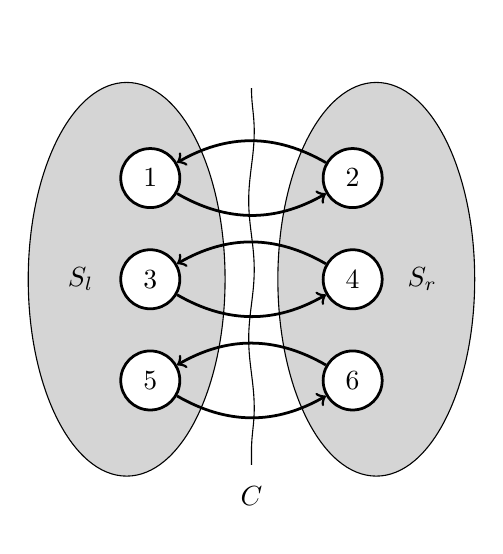
\begin{tikzpicture}[every node/.style={circle,inner sep=0pt,  line width=1pt, minimum size = 0.75cm}]
  \node (center){};
  \node[above = 0.75cm of center] (u){};
  \node[below = 3.25cm of center] (d){$C$};
  \draw[decorate, decoration={snake, segment length=50pt,amplitude=1pt}] (u) to (d);

  \node[draw, left = 0.5cm of center, fill=white] (l1){1};
  \node[draw, right = 0.5cm of center, fill=white] (r1){2};
  \node[draw, below = 0.5cm of l1, fill=white](l2){3};
  \node[draw, below = 0.5cm of r1, fill=white](r2){4};
  \node[draw, below = 0.5cm of l2, fill=white](l3){5};
  \node[draw, below = 0.5cm of r2, fill=white](r3){6};
  \draw [<-, line width=1pt] (l1) edge[bend left] (r1);
  \draw [->, line width=1pt] (l1) edge[bend right] (r1);
  \draw [<-, line width=1pt] (l2) edge[bend left] (r2);
  \draw [->, line width=1pt] (l2) edge[bend right] (r2);
  \draw [<-, line width=1pt] (l3) edge[bend left] (r3);
  \draw [->, line width=1pt] (l3) edge[bend right] (r3);
  \begin{pgfonlayer}{background}
  %\draw[decorate, decoration={random steps,segment length=10pt,amplitude=2pt},rounded corners=5pt, fill=gray!33] ($(l2)-(0.3cm, 0cm)$) ellipse (1.25cm and 2.5cm);
  %\draw[decorate, decoration={random steps,segment length=10pt,amplitude=2pt},rounded corners=5pt, fill=gray!33] ($(r2)+(0.3cm, 0cm)$) ellipse (1.25cm and 2.5cm);
  \draw[fill=gray!33] ($(l2)-(0.3cm, 0cm)$) ellipse (1.25cm and 2.5cm);
  \draw[fill=gray!33] ($(r2)+(0.3cm, 0cm)$) ellipse (1.25cm and 2.5cm);
  \end{pgfonlayer}

  \node[left = 0.1cm of l2] (sl){$S_l$};
  \node[right = 0.1cm of r2] (sr){$S_r$};
  \end{tikzpicture}
  % \hspace{-1em}
  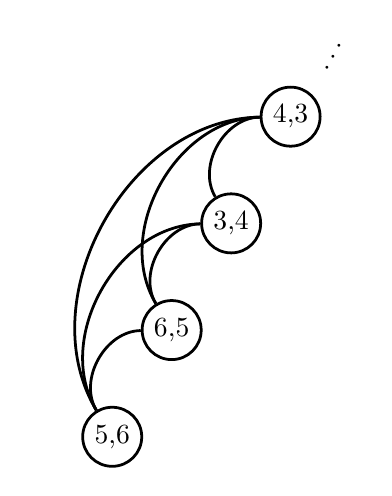
\begin{tikzpicture}[every node/.style={circle,inner sep=0pt,  line width=1pt, minimum size = 0.75cm}]
  \node[draw] (a){5,6};
  \node[draw, above right = 0.8cm and 0.2cm of a] (b){6,5};
  \node[draw, above right = 0.8cm and 0.2cm of b] (c){3,4};
  \node[draw, above right = 0.8cm and 0.2cm of c] (d){4,3};
  \node[above right = 0.2 and 0cm of d] (e){\rotatebox[origin=c]{60.5}{$\cdots$}};
  \draw[-, line width=1pt] (a) edge[bend left=60] (b);
  \draw[-, line width=1pt] (b) edge[bend left=60] (c);
  \draw[-, line width=1pt] (c) edge[bend left=60] (d);
  \draw[-, line width=1pt] (a) edge[bend left=60] (c);
  \draw[-, line width=1pt] (b) edge[bend left=60] (d);
  \draw[-, line width=1pt] (a) edge[bend left=60] (d);
  \end{tikzpicture}
  \hspace{-2.5em}
  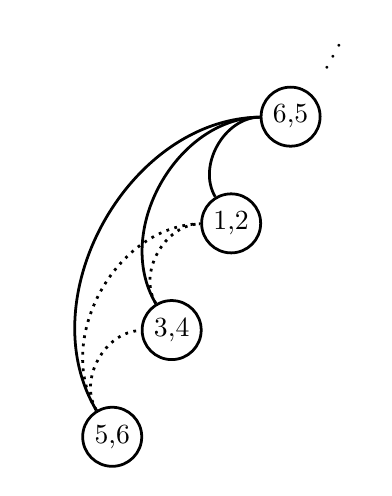
\begin{tikzpicture}[every node/.style={circle,inner sep=0pt,  line width=1pt, minimum size = 0.75cm}]
  \node[draw] (a){5,6};
  \node[draw, above right = 0.8cm and 0.2cm of a] (b){3,4};
  \node[draw, above right = 0.8cm and 0.2cm of b] (c){1,2};
  \node[draw, above right = 0.8cm and 0.2cm of c] (d){6,5};
  \node[above right = 0.2 and 0cm of d] (e){\rotatebox[origin=c]{60.5}{$\cdots$}};
  \draw[dotted, line width=1pt] (a) edge[bend left=60] (b);
  \draw[dotted, line width=1pt] (b) edge[bend left=60] (c);
  \draw[-, line width=1pt] (c) edge[bend left=60] (d);
  \draw[dotted, line width=1pt] (a) edge[bend left=60] (c);
  \draw[-, line width=1pt] (b) edge[bend left=60] (d);
  \draw[-, line width=1pt] (a) edge[bend left=60] (d);
  \end{tikzpicture}
  \caption{On the left is a visualization of a cut in~$G$. In the middle is an arbitrary contraction order which results in no infinite edges after the first four contractions. On the right, the edges in the order are grouped which results in three infinite edges after the first four contractions (shown by the dotted edges). \label{fig:reorder_cut}}
\end{figure}

\subsubsection{Turns with CCH-Potentials}

It is also possible to sidestep the preprocessing and customization slowdown entirely at the cost of some query performance.
As shown in the previous chapter, CH-Potentials are very effective when applied to turn costs and restrictions.
Thus, we can also support turn costs and restrictions in combination with customizability by running bidirectional A* on the expanded graph $G_e$ with CCH-Potentials as the heuristic function.

\section{Experiments}
\label{sec:experiments}

In this section, we present our experimental evaluation.
Our benchmark machine runs openSUSE Leap 15.1 (kernel 4.12.14), and has 192\,GiB of DDR4-2666 RAM and two Intel Xeon Gold 6144 CPUs, each of which has eight cores clocked at 3.5\,Ghz and 8~$\times$~64\,KiB of L1, 8~$\times$~1\,MiB of L2, and 24.75\,MiB of shared L3 cache.
Hyperthreading was disabled and parallel experiments use 16 threads.
Our code is written in C++ and compiled with GCC~8.2.1 using optimization level 3.

We implement our algorithms on top of the existing open-source libraries.
For CCH, we use the implementation from RoutingKit\footnote{\url{https://github.com/RoutingKit/RoutingKit}}.
We extend it by implementing customization for directed hierarchies and the removal of infinite edges.
For the computation of contraction orders, we use InertialFlowCutter\footnote{\url{https://github.com/kit-algo/InertialFlowCutter}}~\cite{GottesburenHUW19} and implement the computation of cut-based orders and the reordering of separator vertices.
We publish our extensions to these projects as pull requests on Github\footnote{\url{https://github.com/RoutingKit/RoutingKit/pull/77}}\footnote{\url{https://github.com/kit-algo/InertialFlowCutter/pull/6}}.
RoutingKit includes an implementation of InertialFlow~\cite{SchildS15} for the computation of contraction orders.
We perform experiments with both InertialFlow and InertialFlowCutter.
As InertialFlow is outperformed by InertialFlowCutter, our evaluation focuses on contraction orders obtained by InertialFlowCutter.

\subparagraph{Inputs and Methodology}

We perform experiments on several graphs with synthetic and real turn cost data.
See Table~\ref{tab:graphs} for an overview.
We use three city-sized instances of the road networks of Chicago~\cite{TNTP}, London and Stuttgart.
The London and Stuttgart instances were provided by PTV\footnote{\url{https://ptvgroup.com}} with real turn restrictions and cost data.
Our biggest benchmark instance is a graph of the road network of Western Europe made publicly available for the Ninth DIMACs implementation challenge~\cite{DemetrescuGJ09} with synthetic turn costs.
% We use two variants of the Europe instance: one with synthetic turn costs and one using proprietary turn restrictions also provided by PTV.
To generate synthetic turn costs, we assign a travel time of 100\,s to all U-turns.
This number does not model a realistic time but a heavy penalty.
All other turns are free.
This model has been suggested in~\cite{DellingGPW17} and found to approximate real-world turn cost effects on the routing sufficiently well.

We perform experiments on the biggest strongly connected component of edge-based model representation of each graph and the induced subgraph on the original graph.
Preprocessing running times are averages over 10 runs, customization running times averages over 100 runs.
We utilize parallelization only for the preprocessing.
All other phases are run sequentially.
For the queries, we perform 1\,000\,000 point-to-point queries where both source and target are edges drawn uniformly at random.
In the edge-based model, these edges correspond to vertices, which we select as source and target.
For the original and compact graph, we use the head vertices of these edges.

\begin{table}
\centering
\caption{
Road networks used for the evaluation our algorithms.
The turns column contains the number of allowed turns.
It corresponds to the number of edges in the edge-based model.
The number of vertices in the edge-based model is equal to the number of edges in the original graph.
}\label{tab:graphs}
\begin{tabular}{llrrrl}
\toprule
           & Source                 &       Vertices &          Edges &          Turns & Turn           \\
           &                        & [$\cdot 10^3$] & [$\cdot 10^3$] & [$\cdot 10^3$] & data           \\
\midrule
Chicago    & TransportationNetworks &           13.0 &           39.0 &          135.3 & 100\,s U-Turns \\
London     & PTV                    &           37.0 &           85.5 &          137.2 & Costs, Restrictions \\
Stuttgart  & PTV                    &          109.5 &          252.1 &          394.2 & Costs, Restrictions \\
Europe     & DIMACS                 &      17\,350.0 &      39\,936.5 &     106\,371.3 & 100\,s U-Turns \\
\bottomrule
\end{tabular}
\end{table}


\begin{table}
\centering
\setlength{\tabcolsep}{5pt}
\caption{
TODO
}\label{tab:preprocessing}
\begin{tabular}{lrrrr}
\toprule
{} &  Ordering & \multicolumn{3}{c}{Contraction} \\ \cmidrule(lr){3-5}
{} &  {} &  Chordal &  Contraction & Dyn. adjacency \\
{} &  {} &  completion & graph \cite{DibbeltSW16} & array \cite{DibbeltSW16} \\
\midrule
Stuttgart &                          0.8 &                          0.0 &          -- &           -- \\
Germany   &                        203.9 &                          1.3 &          -- &           -- \\
Europe    &                        341.2 &                          1.6 &        15.5 &        305.8 \\
\bottomrule
\end{tabular}


\end{table}

\begin{table}
\centering
\setlength{\tabcolsep}{5pt}
\caption{
TODO
}\label{tab:customization}
\begin{tabular}{llrrrrrrrr}
\toprule
& & \multicolumn{4}{c}{Stuttgart [ms]} & \multicolumn{4}{c}{Europe [s]} \\ \cmidrule(lr){3-6} \cmidrule(lr){7-10}
Impl & Threads &     Basic & Perfect & Construct &  Total &  Basic & Perfect & Construct &  Total \\
\midrule
\cite{DibbeltSW16}
& 1           &           &         &           &        &  10.88 &   22.02 & $\approx$ 9.39 & $\approx$ 42.35 \\
& 16          &           &         &           &        & \multicolumn{2}{c}{5.47} & $\approx$ 9.39 & $\approx$ 14.86 \\
\addlinespace
\cite{BuchholdSW19}
& 1           &     20.51 &   20.77 &     48.64 &  89.93 &   5.60 &    6.48 &      9.39 &  21.47 \\
& 16          &      4.91 &    4.41 &      4.35 &  13.66 &   1.11 &    0.63 &      0.80 &   2.54 \\
\addlinespace
{[ours]}
& 1           &     19.85 &   18.95 &     10.33 &  49.13 &   4.09 &    4.72 &      1.95 &  10.76 \\
& 2           &     11.34 &    9.90 &      5.69 &  26.93 &   2.05 &    2.42 &      0.99 &   5.46 \\
& 4           &      7.39 &    5.65 &      3.57 &  16.61 &   1.22 &    1.26 &      0.54 &   3.02 \\
& 8           &      5.70 &    3.51 &      2.46 &  11.67 &   0.81 &    0.69 &      0.35 &   1.86 \\
& 16          &      6.25 &    3.10 &      2.59 &  11.94 &   0.58 &    0.37 &      0.30 &   1.25 \\
\bottomrule
\end{tabular}


\end{table}

\begin{table}
\centering
\setlength{\tabcolsep}{5pt}
\caption{
TODO
}\label{tab:queries}
\begin{tabular}{llrrrrrrrr}
\toprule
& {}      & \multicolumn{3}{c}{Search space}     & \multicolumn{4}{c}{Running time [$\mu$s]}               & \# Path    \\ \cmidrule(lr){3-5} \cmidrule(lr){6-9}
& {} & \multirow{2}{*}{Vertices} & \multicolumn{2}{c}{Edges} & \multicolumn{2}{c}{Distance} & \multicolumn{2}{c}{Path} & Vertices \\ \cmidrule(lr){4-5} \cmidrule(lr){6-7} \cmidrule(lr){8-9}
\multicolumn{2}{r}{Perfect Customization} & &                  \xmark &      \cmark &           \xmark &   \cmark &     \xmark &   \cmark &         \\
\midrule
Stuttgart & Travel time &                    216.4 &            8\,846.5 &    3\,837.1 &            22.9 &   14.5 &       5.6 &    5.4 &             185.9 \\
       & Geo distance &                    216.4 &            8\,888.6 &    3\,303.3 &            22.2 &   13.0 &       4.4 &    4.2 &             149.8 \\
\addlinespace
Germany & Travel time &                   1\,277.9 &          274\,113.1 &   78\,474.2 &           442.0 &  163.2 &     234.6 &  134.4 &            4\,681.0 \\
       & Heavy traffic &                   1\,277.9 &          274\,478.3 &   85\,298.9 &           435.0 &  174.2 &     241.7 &  179.5 &            5\,363.4 \\
       & Geo distance &                   1\,277.9 &          274\,788.5 &  131\,985.4 &           438.3 &  246.3 &     383.4 &  336.2 &            6\,174.7 \\
\addlinespace
Europe & Travel time &                   1\,041.2 &          186\,006.5 &   69\,312.9 &           300.2 &  137.5 &      95.9 &   71.3 &            1\,389.8 \\
       & Geo distance &                   1\,041.2 &          185\,701.3 &   92\,616.8 &           303.3 &  177.9 &     281.3 &  252.9 &            3\,158.9 \\
\bottomrule
\end{tabular}


\end{table}

\subparagraph{Edge-based model}

\begin{table}[tb]
\parbox{.5\linewidth}{
\setlength{\tabcolsep}{2.8pt}
\centering
\caption{
Performance results for different contraction orders on each graph.
We report the number of edges in the augmented graph and running times for preprocessing, customization, and queries.
\emph{Orig.} denotes the baseline on the nonturn/compact graph.
The other three orders are for the edge-based model.
\emph{Deri.} indicates the derived order, \emph{Edge} the order computed on the expanded graph, \emph{Cut} the order obtained by ordering edges in the original graph.
}\label{tab:orders}
\begin{tabular}{llrrrr}
\toprule
       & &      CCH Edges & Prepro. & Custom. &    Query \\
       & & [$\cdot 10^3$] &     [s] &    [ms] & [$\mu$s] \\
\midrule
\parbox[t]{3mm}{\multirow{4}{*}{\rotatebox[origin=c]{90}{Chicago}}}
& Orig. &            118 &                  0.2 &                               6 &              18 \\
& Deri. &           1\,439 &                  0.2 &                             155 &             150 \\
& Edge &            819 &                  1.1 &                              50 &              60 \\
& Cut &            852 &                  0.2 &                              51 &              57 \\
\addlinespace
\parbox[t]{3mm}{\multirow{4}{*}{\rotatebox[origin=c]{90}{London}}}
& Orig. &            182 &                  0.3 &                               7 &              20 \\
& Deri. &           1\,199 &                  0.3 &                              85 &             111 \\
& Edge &            767 &                  1.1 &                              37 &              52 \\
& Cut &            840 &                  0.3 &                              40 &              51 \\
\addlinespace
\parbox[t]{3mm}{\multirow{4}{*}{\rotatebox[origin=c]{90}{Stuttgart}}}
& Orig. &            362 &                  0.5 &                              11 &              16 \\
& Deri. &           2\,145 &                  0.6 &                              94 &              79 \\
& Edge &           1\,607 &                  2.4 &                              58 &              41 \\
& Cut &           1\,680 &                  0.9 &                              60 &              37 \\
\addlinespace
\parbox[t]{3mm}{\multirow{4}{*}{\rotatebox[origin=c]{90}{Europe}}}
& Orig. &          53\,521 &                182.3 &                            2\,349 &             187 \\
& Deri. &         414\,615 &                202.1 &                           29\,787 &            1\,561 \\
& Edge &         311\,213 &               2\,321.1 &                           14\,787 &             524 \\
& Cut &         331\,794 &                256.3 &                           14\,751 &             577 \\
\bottomrule
\end{tabular}
}
\quad
\parbox{.45\linewidth}{
\setlength{\tabcolsep}{3pt}
\centering
\caption{
Performance impact of different optimizations on each graph.
We report the number of triangles enumerated during the customization as well as customization and query running times.
All configurations use a cut-based contraction order.
Directed hierarchies imply the removal of infinite shortcuts and reordering separator vertices builds on both directed hierarchies and the removal of infinite shortcuts.
}\label{tab:opt}
\begin{tabular}{llrrr}
\toprule
 & &      Triangles & Custom. &    Query \\
 & & [$\cdot 10^6$] &    [ms] & [$\mu$s] \\
\midrule
\parbox[t]{3mm}{\multirow{4}{*}{\rotatebox[origin=c]{90}{Chicago}}}
& None &           21.6 &                              51 &              57 \\
& Infinity &           19.6 &                              48 &              56 \\
& Directed &           13.3 &                              28 &              41 \\
& Reorder &            8.2 &                              20 &              31 \\
\addlinespace
\parbox[t]{3mm}{\multirow{4}{*}{\rotatebox[origin=c]{90}{London}}}
& None &           12.9 &                              40 &              51 \\
& Infinity &           11.0 &                              36 &              51 \\
& Directed &            7.7 &                              23 &              40 \\
& Reorder &            4.8 &                              18 &              30 \\
\addlinespace
\parbox[t]{3mm}{\multirow{4}{*}{\rotatebox[origin=c]{90}{Stuttgart}}}
& None &           11.4 &                              60 &              37 \\
& Infinity &            8.5 &                              53 &              37 \\
& Directed &            6.2 &                              36 &              30 \\
& Reorder &            4.4 &                              32 &              22 \\
\addlinespace
\parbox[t]{3mm}{\multirow{4}{*}{\rotatebox[origin=c]{90}{Europe}}}
& None &         3\,955.7 &                           14\,751 &             577 \\
& Infinity &         3\,413.6 &                           13\,942 &             582 \\
& Directed &         2\,319.7 &                            9\,590 &             407 \\
& Reorder &         1\,514.2 &                            8\,180 &             306 \\
\bottomrule
\end{tabular}
}
\end{table}

We evaluate the impact of different contraction orders on the performance of the different phases and the size of the augmented graph.
Preprocessing includes both computing the order and the contraction but is dominated by the ordering.
Table~\ref{tab:orders} depicts the results.
Incorporating turns has a significant impact on the running time of all phases of CCH.
The number of edges in the hierarchy grows at least by a factor of four to up to more than an order of magnitude.
The derived order performs the worst on all instances.
On Chicago, the customization slows down by a factor of 25.
On the other instances, the slowdown is about an order of magnitude.
The slowdown for queries is not as strong but still significant (by a factor of 5 to 8).
Only the preprocessing stays comparatively fast as it is dominated by the order computation, which can run on the unmodified original graph.
We conclude that this approach is not feasible.

With the edge-based order, we achieve a better order at the cost of additional preprocessing time.
The slowdown compared to a nonturn CCH is reduced to a factor of five for the customization phase, for queries to 2.5 to 3.
However, preprocessing takes up to an order of magnitude longer.
Orders computed by InertialFlow are generally worse than InertialFlowCutter orders (the customization is a factor 1.3 to 1.5 slower) and on graphs of the edge-based model this difference becomes even more pronounced (factor 1.3 to 2.8).
Consequentially, we focus on InertialFlowCutter orders.

Cut orders achieve the best trade-off between the running times of the different phases.
Customization and query performance is roughly the same as with an edge-based order.
The preprocessing slowdown is well below a factor of two for all graphs.
InertialFlowCutter has certain optimizations which find optimal vertex orders for certain subclasses of graphs.
We did not implement these optimizations for cut-based orders.
We expect that implementing them would close the gap in quality between edge-based and cut-based orders.
% why slower than orig?
%   because need more cuts
%   + missing IFC optimization magic

In Table~\ref{tab:opt}, we report performance results depending on the additional optimizations applied.
All configurations use cut-based orders.
% Thus, preprocessing times are the same for all configurations.
We also report the number of triangles enumerated during the customization as the triangle enumeration dominates the customization running time.
The impact of the optimizations is similar across all instances.
All optimizations combined roughly achieve a speedup of two on both customization and queries.
Removing undirected infinite shortcuts alone yields only small improvements.
Combining this with directed hierarchies and removing all directed infinite shortcuts has a much bigger impact.
This impact can be further amplified by reordering separator vertices, which produces even more infinite shortcuts.
Note that the work per triangle is different for directed hierarchies.
For undirected hierarchies, each triangle will be enumerated once and both directed triangles will be relaxed at once.
For directed hierarchies, however, both directions will be enumerated separately.
Thus, for undirected hierarchies, the number of relaxation operations is twice the number of enumerated triangles and the reduction achieved by directed hierarchies even greater.
It is noteworthy that even though our optimizations primarily aim for the customization running time, we also achieve a significant speedup for query running times.
The removal of infinite edges also reduces the number of edges in the query search space.

\subparagraph{Comparison with related work}

\begin{table}
\centering
\caption{
Performance of Dijkstra, CH, CRP and CCH in the compact model, in the edge-based model as is and with our optimizations (Edge-based*) on Europe with and without turns.
Preprocessing and customization were executed in parallel, queries sequentially.
For CH and CRP we list unscaled results as reported in \cite{DellingGPW17}.
}\label{tab:related_work}
\begin{tabular}{l@{\hskip4pt}crrrlrrr}
\toprule
{}                        &                                      & \multicolumn{3}{c}{No turns}                                           & \multicolumn{4}{c}{Turns}                  \\
                                                                   \cmidrule(lr){3-5}                                                       \cmidrule(lr){6-9}
{}                        &                                      &             Prepro.  &            Custom. &                    Queries & Repr.      & Prepro. & Custom. &   Queries \\
{}                        &                                      &                 [s]  &                [s] &                       [ms] &            &     [s] &     [s] &      [ms] \\
\midrule
\multirow{2}{*}{Dijkstra} &                                      &   \multirow{2}{*}{-} & \multirow{2}{*}{-} & \multirow{2}{*}{1\,061.52} & Edge-based &       - &       - &  2\,674.72 \\
                          &                                      &                      &                    &                            &    Compact &       - &       - & 12\,699.32 \\
\addlinespace
\multirow{2}{*}{CH}       & \multirow{2}{*}{\cite{DellingGPW17}} & \multirow{2}{*}{109} & \multirow{2}{*}{-} &      \multirow{2}{*}{0.11} & Edge-based &  1\,392 &       - &       0.19 \\
                          &                                      &                      &                    &                            &    Compact &  1\,753 &       - &       2.27 \\
\addlinespace
CRP                       & \cite{DellingGPW17}                  &                  654 &               1.05 &                       1.65 &    Compact &     654 &    1.10 &       1.67 \\
\addlinespace
\multirow{2}{*}{CCH}      &                                      & \multirow{2}{*}{221} & \multirow{2}{*}{1.43} &   \multirow{2}{*}{0.15} & Edge-based &  2\,758 &    7.31 &       0.26 \\
                          &                                      &                      &                    &                            & Edge-based* &    277 &    4.05 &       0.34 \\
\bottomrule
\end{tabular}
\end{table}

Table~\ref{tab:related_work} summarizes our results and depicts them in comparison to running times achieved by competing approaches as reported in~\cite{DellingGPW17}.
The experiments were performed on the publicly available Europe instance which is the only instance also considered in related work.
Our experiments were conducted on a newer machine.
Thus, the absolute numbers are not perfectly comparable.
Using the comparison methodology from~\cite{BastDGMPSWW16}, the numbers from~\cite{DellingGPW17} should scaled down by a factor of 0.79.
We observe that incorporating turns has a strong impact on all algorithms except CRP.
Dijkstra becomes at least 2.5 times slower.
CH queries remain comparatively fast (at least on the edge-based model), but preprocessing slows down by more than an order of magnitude.
The CRP nonturn variant is realized as free turns in the compact model which explains why incorporating turns leaves the performance unaffected.
% By using the simplified model, CRP could likely be accelerated further.
While CCH achieves faster running times than CRP in all phases on nonturn graphs, without our modifications, it is outperformed by CRP on graphs with turns.
However, when using cut-based orders and all optimizations, CCH again outperforms CRP.
CCH with the compact model is outperformed by the optimized edge-based variant in all phases.
Note that both the CRP and CCH customization times can be further decreased through parallelization and by two related techniques known as microcode~\cite{DellingW13} (for CRP) and triangle preprocessing~\cite{DibbeltSW16} (for CCH).
However, both techniques require significantly more space, and we choose not to use them to keep the space requirement low.

% dijkstra scaling factors (2.5-3)
% turn dijkstra slowdown (2-3)
% CH: turn slowdown by more than order of magnitude for prepro
%   queries not as bad, at least for edge based.
%   compact even worse, also for queries, but less space
% CRP slow but robust
% customization for both CRP and CCH can be speed up further by parallelization.


\begin{figure}
\centering
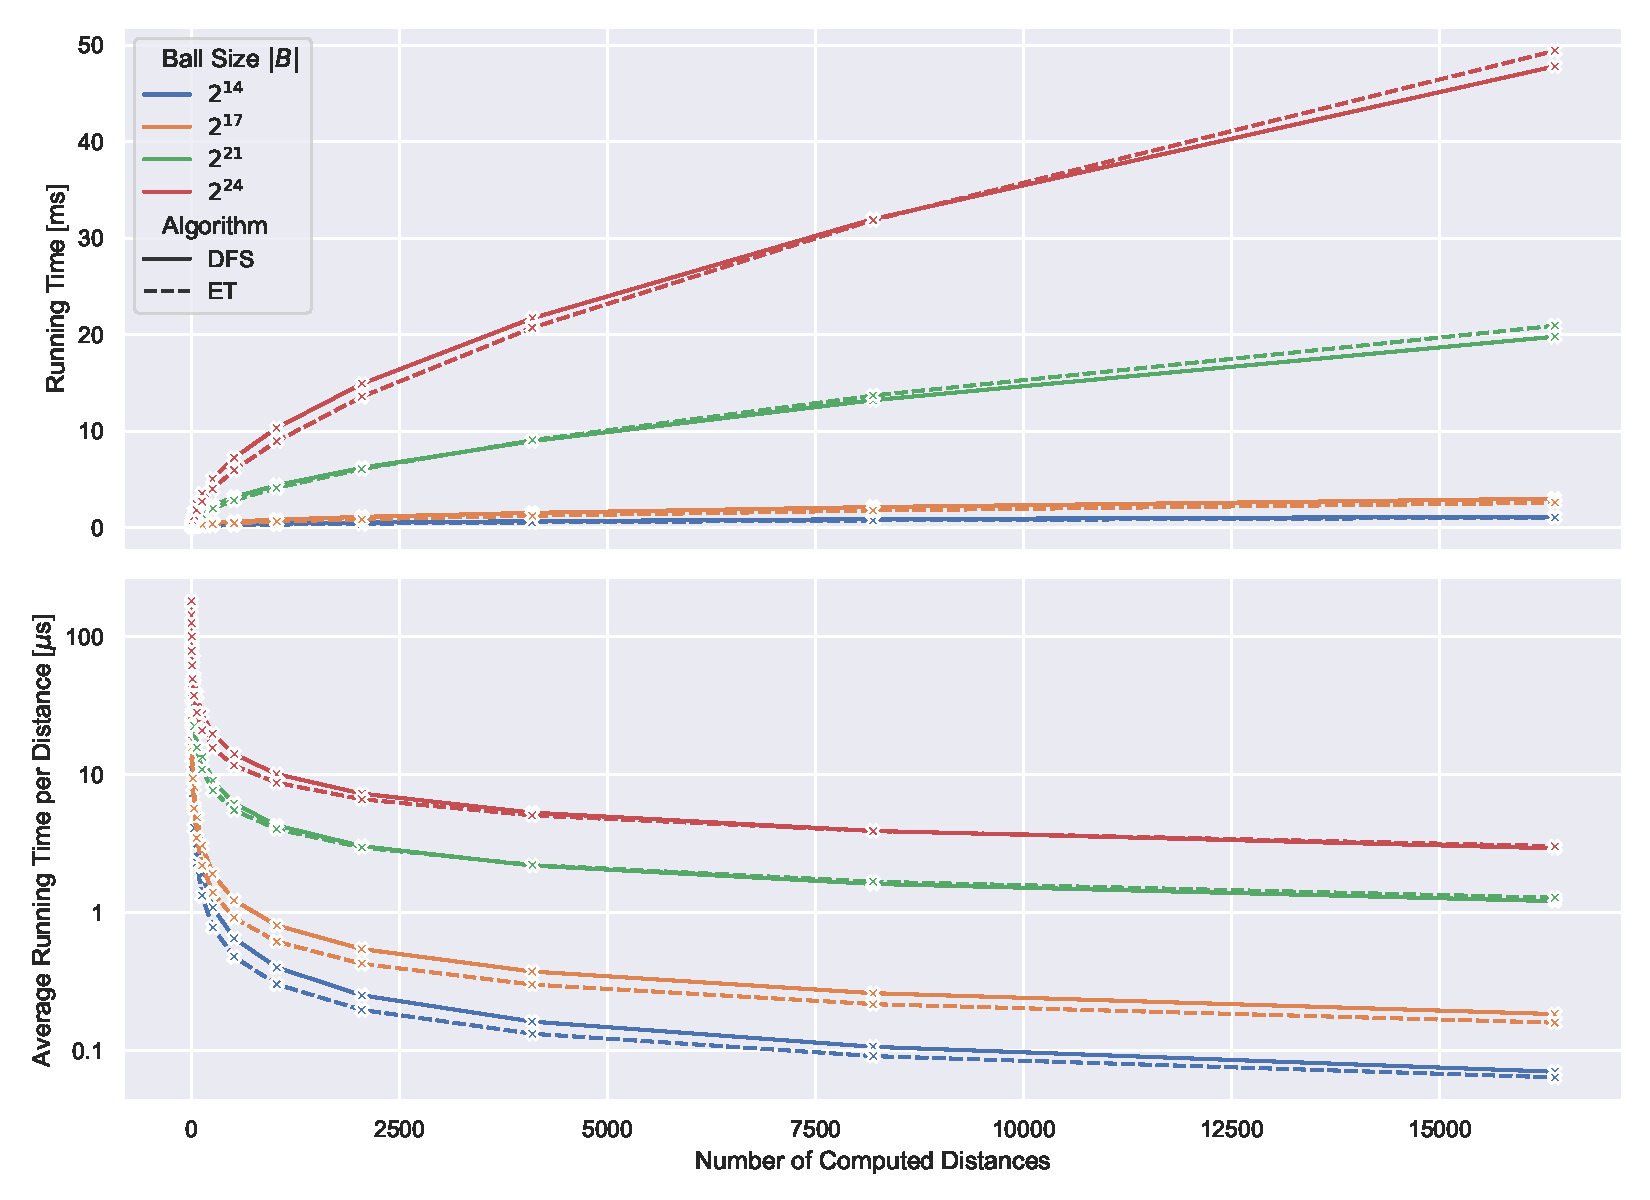
\includegraphics[width=\linewidth]{fig/lazy_rphast_et_vs_dfs.pdf}
\caption{
TODO
}\label{fig:et_vs_dfs}
\end{figure}

\begin{figure}
\centering
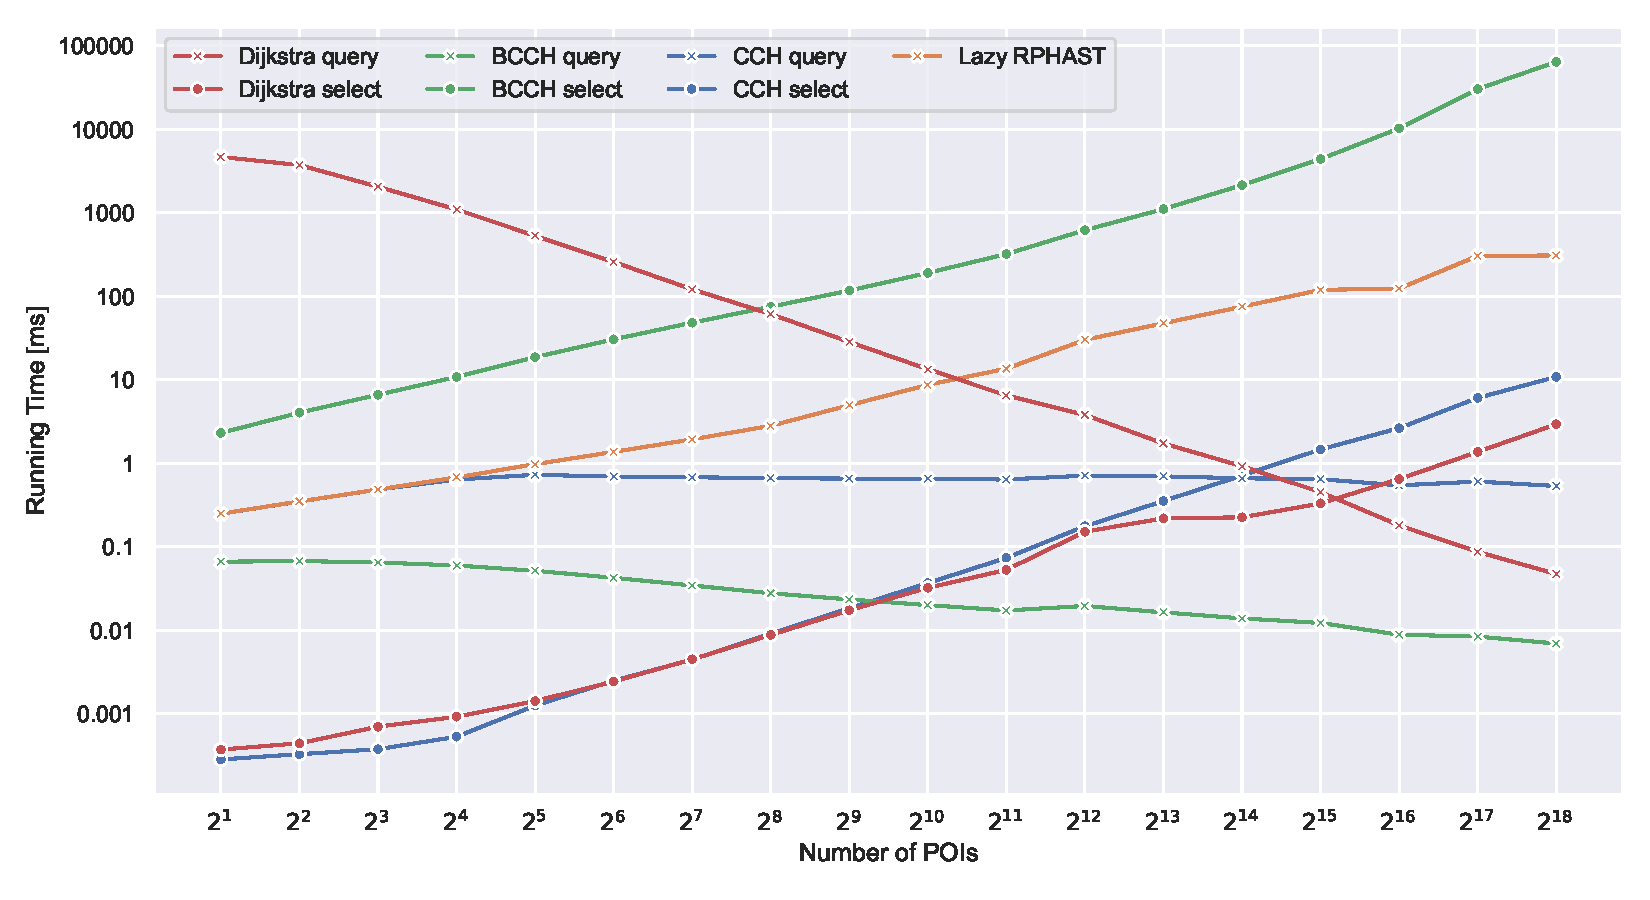
\includegraphics[width=\linewidth]{fig/knn.pdf}
\caption{
TODO
}\label{fig:knn}
\end{figure}

\section{Conclusion}
\label{sec:conclusion}

We incorporated turn costs and restrictions into CCH. We presented several straightforward yet effective optimizations that bring preprocessing and customization times on the expanded graph close to those achieved on the simplified graph. Preprocessing now takes similar time on the simplified and expanded graph, and customization on the expanded graph is only roughly three times slower (down from up to an order of magnitude, e.g., on Chicago).

Adapting CCH to the compact model was much harder. We observed that CCH and the compact model do not match well. CCH relies heavily on concepts for undirected graphs, whereas the compact model is inherently directed. Moreover, shortcuts built from more than two edges are an issue for CCH customization, where there is no notion of graph searches. Consequently, our experiments showed that the CCH implementation tailored to expanded graphs significantly outperforms the one for compact graphs.

\bibliography{References}

\end{document}
